%!TEX root = /Users/jakubkonka/Thesis/Thesis.tex
\chapter{Indirect Analysis of Network Selection Mechanism}
\label{cha:indirect}

In this chapter, the bidding problem described in Section~\ref{sec:problem_definition_and_assumptions_direct} is transformed from a bidding problem with symmetric cost (or type) distributions into a bidding problem with asymmetric cost distributions. This type of bidding problems has already been researched by the economic community, both in a very specific setting (two bidders, specific cost distributions) \cite{KaplanZamir2007,MaskinRiley2000}, and in a very general setting ($n$ bidders, arbitrary cost distributions) \cite{Lebrun1999,Lebrun2006}, and hence there exist results that are applicable to the problem at hand.

In the first instance, it is showed how the problem can be restated into a bidding problem with asymmetric cost distributions. The discussion then proceeds to characterising the equilibrium bidding strategies (their existence and uniqueness) in the generic case; that is, with an arbitrary number of network operators and an arbitrary distribution of costs. The equilibrium bidding strategies are then explicitly derived in the restricted case; that is, with the number of network operators restricted to two and the costs uniformly distributed. Finally, the chapter concludes with the presentation of three numerical methods that can be used to numerically approximate the equilibrium bidding strategies in the case of more than two network operators characterised by uniform distributions of costs.

\section{Problem Restatement} % (fold)
\label{sec:problem_restatement_indirect}
In order to transform the problem, recall the utility function for each network operator~$i$
\begin{equation}
  u_i(b,c,r) = \left\{
  \begin{array}{l l}
    b_i-c_i & \;\textrm{if } wb_i + (1-w)r_i < \displaystyle\min_{j\neq i}[wb_j + (1-w)r_j],\\
    0 & \;\textrm{if } wb_i + (1-w)r_i > \displaystyle\min_{j\neq i}[wb_j + (1-w)r_j],
  \end{array}\right.
\end{equation}
and let
\begin{equation}
  \label{eq:b_hat_indirect}
  \hat{b}_i = wb_i + (1-w)r_i \quad\textrm{for all } i\in N.
\end{equation}
Solving Equation~\eqref{eq:b_hat_indirect} for $b_i$ yields
\begin{equation}
  \label{eq:b_from_b_hat_indirect}
  b_i = \frac{\hat{b}_i - (1-w)r_i}{w}, \quad w\neq 0.
\end{equation}
Substituting Equation~\eqref{eq:b_from_b_hat_indirect} back into the utility function yields
\begin{equation}
  u_i(\hat{b},c,r) = \left\{
  \begin{array}{l l}
    \displaystyle\frac{1}{w}\left[\hat{b}_i-(wc_i + (1-w)r_i)\right] & \;\textrm{if } \hat{b}_i < \displaystyle\min_{j\neq i}\hat{b}_j,\\[2ex]
    0 & \;\textrm{if } \hat{b}_i > \displaystyle\min_{j\neq i}\hat{b}_j.
  \end{array}\right.
\end{equation}
Further let
\begin{equation}
  \label{eq:cost_hat_indirect}
  \hat{c}_i = wc_i + (1-w)r_i \quad\textrm{for all } i\in N,
\end{equation}
then the utility function simplifies to
\begin{equation}
  \label{eq:sellers_utility_hat_full_indirect}
  u_i(\hat{b},\hat{c}) = \left\{
  \begin{array}{l l}
    \displaystyle\frac{1}{w}\left(\hat{b}_i-\hat{c}_i\right) & \;\textrm{if } \hat{b}_i < \displaystyle\min_{j\neq i}\hat{b}_j,\\[2ex]
    0 & \;\textrm{if } \hat{b}_i > \displaystyle\min_{j\neq i}\hat{b}_j.
  \end{array}\right.
\end{equation}

The rest of this thesis concentrates on the utility function with the scaling factor, $\displaystyle\sfrac{1}{w}$, omitted; that is, let
\begin{equation}
  \label{eq:sellers_utility_hat_indirect}
    \hat{u}_i(\hat{b},\hat{c}) = w\cdot u_i(\hat{b}, \hat{c})
\end{equation}
for all $i\in N$. In fact, it can be noted that the pure-strategy Bayesian Nash equilibrium for the auction with utility function in Equation~\eqref{eq:sellers_utility_hat_indirect} constitutes an equilibrium for the auction with utility function in Equation~\eqref{eq:sellers_utility_hat_full_indirect}. Formally,
\begin{proposition}
\label{prop:equivalence_of_utilities_indirect}
Suppose $(\hat{b}_1^*, \ldots, \hat{b}_n^*)$ is a pure-strategy Bayesian Nash equilibrium profile for an auction with the utility function
\begin{equation}
  \hat{u}_i(\hat{b}_i,\hat{c}_i,\hat{b}_{-i},\hat{c}_{-i}) = \left\{
  \begin{array}{l l}
    \displaystyle\left(\hat{b}_i-\hat{c}_i\right) & \;\textrm{if}\quad\hat{b}_i < \displaystyle\min_{j\neq i}\hat{b}_j,\\[2ex]
    0 & \;\textrm{if}\quad\hat{b}_i > \displaystyle\min_{j\neq i}\hat{b}_j.
  \end{array}\right.
\end{equation}
Then, the same profile constitutes an equilibrium for an auction with the utility function
\begin{equation}
  u_i(\hat{b}_i,\hat{c}_i,\hat{b}_{-i},\hat{c}_{-i}) = \frac{1}{w}\cdot \hat{u}_i(\hat{b}_i,\hat{c}_i,\hat{b}_{-i},\hat{c}_{-i}).
\end{equation}
\end{proposition}

In order to avoid ambiguity, $\hat{c}_i$ will be referred to as cost-hat and $\hat{b}_i$ as bid-hat, while $c_i$ will still be referred to as cost and $b_i$ as bid. Note, moreover, that since both $w$ and $r_i$ are assumed to be given to the network operators (i.e., they cannot directly modify their values), the costs-hat and bids-hat are simply convex (and hence, linear) combinations involving costs and bids respectively (Equations~\eqref{eq:b_hat_indirect}~and~\eqref{eq:cost_hat_indirect}). Therefore, a network operator bidding their cost-hat is equivalent to bidding their cost.

As a result of this transformation, the costs-hat, $\hat{c}_i$, for each network operator $i$ are distributed over the interval
\begin{equation}
  \hat{c}_i\in [(1-w)r_i, (1-w)r_i + w]= [\underline{\hat{c}}_i, \bar{\hat{c}}_i]
\end{equation}
since $c_i\in [0,1]$ for all $i\in N$. Note, moreover, that for all $i\in N$
\begin{equation}
  [\underline{\hat{c}}_i, \bar{\hat{c}}_i] \subset [0,1]
\end{equation}
since $w\in (0,1)$ and $r_i\in [0,1]$, and in particular, if $w=1$
\begin{equation}
  [\underline{\hat{c}}_i, \bar{\hat{c}}_i] = [0,1].
\end{equation}
Therefore, in terms of costs-hat, the network operators are \emph{ex ante} asymmetric; that is, due to differing domains of costs-hat between the network operators, the probability distributions will have differing supports.

With these results at hand, the discussion can proceed with the characterisation of the equilibrium bidding strategies in the generic case, which is the subject of the next section.
% section problem_restatement_indirect (end)

\section{Generic Case} % (fold)
\label{sec:generic_case_indirect}
In the generic case, with arbitrary probability distributions of costs and $n\ge 2$ network operators, recall that: if $w=0$, then Proposition~\ref{prop:special_case_w_0_direct} holds; if $w=1$, then Proposition~\ref{prop:special_case_w_1_direct} holds; and if $r_i=r_j$ for all $i,j\in N$ such that $i\neq j$, then Corollary~\ref{cor:special_case_r_i_r_j_direct} holds. Therefore, it suffices to consider only the case when $w\in (0,1)$.

Firstly, note that under the generic assumptions specified in Section~\ref{sec:problem_definition_and_assumptions_direct} and $w\in (0,1]$, the problem satisfies the following regularity conditions.
\begin{proposition}[Regularity Conditions]
\label{prop:regularity_conditions_indirect}
Let $F_i$ be the distribution function of $\hat{c}_i$ for all $i\in N$, and suppose $w\in (0,1]$. Then,
\begin{enumerate}
  \item the support of $F_i$ is an interval ${[\underline{\hat{c}}_i, \bar{\hat{c}}_i]}$;
  \item $F_i$ is differentiable over ${(\underline{\hat{c}}_i, \bar{\hat{c}}_i]}$ with a derivative $f_i$ locally bounded away from zero over this interval; and
  \item $F_i$ is atomless.
\end{enumerate}
\end{proposition}

The regularity conditions in Proposition~\ref{prop:regularity_conditions_indirect} correspond to the regularity assumptions on type distributions put forward by Lebrun~\cite{Lebrun2006} (cf. Assumptions~A.1 in~\cite{Lebrun2006}). Therefore, since the problem satisfies Lebrun's assumptions, his results are applicable.

Further assume that
\begin{assumptions}
\label{ass:assumptions_generic_indirect}
Assume that
\begin{enumerate}
  \item $w\in(0,1)$;
  \item there exists $i\in N$ such that $r_i\neq r_j$ for all $i\neq j$ and $j\in N$; and
  \item without loss of generality, let network operator 1 be characterized by the lowest reputation rating; that is, $r_1 \leq r_i$ for all $i\in N$ such that $i\neq 1$. If there exists $j\in N$ such that $j\neq 1$ and $r_1 = r_j$, then it is further assumed that there exists $\delta > 0$ such that $F_i$ is strictly log-concave over $(\bar{\hat{c}}_1 - \delta, \bar{\hat{c}}_1)\cap (\underline{\hat{c}}_i, \bar{\hat{c}}_i)$ for all $i\in N$.
\end{enumerate}
\end{assumptions}

In equilibrium, the bids of each network operator equal $\hat{b}_i = \hat{b}_i(\hat{c}_i)$, where $\hat{b}_i$ is the equilibrium bidding function. Denote by $\hat{c}_i(\hat{b}_i)= \hat{b}_i^{-1}(\hat{b}_i)$ an inverse equilibrium bidding function for each network operator $i\in N$. Therefore, the expected utility for each network operator $i\in N$ can be written as
\begin{align}
  \label{eq:def_expected_utility_indirect}
  \Pi_i(\hat{b}_i,\hat{c}_i,\hat{b}_{-i},\hat{c}_{-i})
  &= (\hat{b}_i - \hat{c}_i)P\{\textrm{winning}\mid\hat{b}_i\}\\ \nonumber
  &= (\hat{b}_i - \hat{c}_i)Q_i(\hat{b}_i),
\end{align}
where
\begin{equation}
Q_i(\hat{b}_i) = \prod_{j\neq i}\left( 1 - F_j(\hat{c}_j(\hat{b}_i)) \right)
\end{equation}
is the probability that network operator $i$ is the lowest bidder.

The first order condition for maximising network operator $i$'s expected utility is
\begin{equation}
  \label{eq:foc_indirect}
  \frac{d}{d\hat{b}_i}\Pi_i(\hat{b}_i,\hat{c}_i,\hat{b}_{-i},\hat{c}_{-i}) = Q_i(\hat{b}_i) + (\hat{b}_i - \hat{c}_i)\cdot\frac{d}{d\hat{b}_i}Q_i(\hat{b}_i) = 0,
\end{equation}
where
\begin{equation}
  \frac{d}{d\hat{b}_i}Q_i(\hat{b}_i) = (-1)\sum_{j\neq i} f_j(\hat{c}_j(\hat{b}_i))\frac{d}{d\hat{b}_i}\hat{c}_j(\hat{b}_i)\prod_{k\neq j} \left( 1 - F_k(\hat{c}_k(\hat{b}_i)) \right).
\end{equation}

Noting that in equilibrium $\hat{c}_i = \hat{c}_i(\hat{b}_i)$, letting $\hat{b}_i = b$, and rearranging terms in Equation~\eqref{eq:foc_indirect} yields
\begin{align}
  \label{eq:foc_simplified_indirect}
  \frac{1}{b - \hat{c}_i(b)} 
  &= \frac{\sum_{j\neq i} f_j(\hat{c}_j(b))\frac{d}{db}\hat{c}_j(b)\prod_{k\neq j} \left( 1 - F_k(\hat{c}_k(b)) \right)}{\prod_{j\neq i} \left( 1 - F_j(\hat{c}_j(b)) \right)}\nonumber \\[2ex]
  &= \sum_{j\neq i}\frac{f_j(\hat{c}_j(b))}{1 - F_j(\hat{c}_j(b))}\cdot\frac{d}{db}\hat{c}_j(b).
\end{align}
Summing Equation~\eqref{eq:foc_simplified_indirect} over all $n$ network operators yields
\begin{equation}
  \label{eq:foc_summed_indirect}
  \frac{1}{n-1}\sum_{i=1}^n \frac{1}{b - \hat{c}_i(b)} = \sum_{i=1}^n \frac{f_i(\hat{c}_i(b))}{1 - F_i(\hat{c}_i(b))}\cdot\frac{d}{db}\hat{c}_i(b).
\end{equation}
Subtracting Equation~\eqref{eq:foc_simplified_indirect} from \eqref{eq:foc_summed_indirect} yields 
\begin{equation}
  \frac{1}{n-1}\sum_{i=1}^n \frac{1}{b - \hat{c}_i(b)} - \frac{1}{b - \hat{c}_i(b)} = \frac{f_i(\hat{c}_i(b))}{1 - F_i(\hat{c}_i(b))}\cdot\frac{d}{db}\hat{c}_i(b)
\end{equation}
which leads to the system of nonlinear ordinary differential equations (ODE)
\begin{equation}
  \frac{d}{db}\hat{c}_i(b) = \frac{1 - F_i(\hat{c}_i(b))}{f_i(\hat{c}_i(b))}\left[ \frac{1}{n-1}\sum_{i=1}^n \frac{1}{b-\hat{c}_i(b)} - \frac{1}{b-\hat{c}_i(b)} \right]
\end{equation}
for $i=1,2,\dotsc,n$. As will be shown briefly, there exists a unique set of inverse bidding functions that satisfy the system and constitute a pure-strategy Bayesian Nash equilibrium where network operators submit at least their costs-hat. Firstly, few concepts need to be defined (cf.~Definitions 1, 2 and 3 in Lebrun~\cite{Lebrun2006}).

\begin{define}[Upper bound on bids]
\label{def:upper_bound_bids_indirect}
Let Assumptions~\ref{ass:assumptions_generic_indirect} be satisfied. Then, the upper bound on bids is defined as follows
\begin{equation}
  \label{eq:upper_bound_bids_indirect}
  \bar{\hat{b}} = \min\arg\max_{b\in[\bar{\hat{c}}_1, \bar{\hat{c}}_2]}(b - \bar{\hat{c}}_1)\prod_{i>1}\left( 1 - F_i(b) \right).
\end{equation}
\end{define}

\begin{define}[Feasible bidders]
\label{def:feasible_bidders_indirect}
Let Assumptions~\ref{ass:assumptions_generic_indirect} be satisfied. Let $J$ denote the set of feasible bidders. Then, $J$ is a subset of $N$ such that
\begin{equation}
  J = \left\{j \:\middle\vert\: 1\leq j\leq n \textrm{ and } \underline{\hat{c}}_j < \bar{\hat{b}}\right\}.
\end{equation}
Furthermore, let $n' = |J|$.
\end{define}

\begin{define}[Characterisation of lower bound on bids]
\label{def:lower_bound_bids_indirect}
Let Assumptions~\ref{ass:assumptions_generic_indirect} be satisfied. Then,
\begin{enumerate}
  \item For all $\underline{\hat{b}}\in (\underline{\hat{c}}_2, \bar{\hat{b}})$, there exists one and only one $k(\underline{\hat{b}})\in \{2,\dotsc,n\}$ such that $\underline{\hat{c}}_{k(\underline{\hat{b}})} < \underline{\hat{b}}$ and
  \begin{equation}
    \frac{1}{\underline{\hat{b}} - \underline{\hat{c}}_{k(\underline{\hat{b}})}}\leq \frac{1}{k(\underline{\hat{b}}) - 1}\sum_{i=1}^{k(\underline{\hat{b}})}\frac{1}{\underline{\hat{b}} - \underline{\hat{c}}_i},
  \end{equation}
  and if $\underline{\hat{c}}_{k(\underline{\hat{b}})+1} < \underline{\hat{b}}$ (and $k(\underline{\hat{b}}) < n$)
  \begin{equation}
    \frac{1}{k(\underline{\hat{b}}) - 1}\sum_{i=1}^{k(\underline{\hat{b}})}\frac{1}{\underline{\hat{b}} - \underline{\hat{c}}_i} < \frac{1}{\underline{\hat{b}} - \underline{\hat{c}}_{k(\underline{\hat{b}})+1}}.
  \end{equation}
  The proof of this assertion can be found in Lebrun~\cite{Lebrun2004} (see Lemma A4.1, Appendix 4).
  \item For all $\underline{\hat{b}}\in (\underline{\hat{c}}_2, \bar{\hat{b}})$, let $\hat{c}(\underline{\hat{b}})$ be defined as follows
  \begin{equation}
  \label{eq:lower_bound_bids_cost_indirect}
    \hat{c}(\underline{\hat{b}}) = \underline{\hat{b}} - \sfrac{\left(k(\underline{\hat{b}})-1\right)}{\left(\sum_{i=1}^{k(\underline{\hat{b}})} \frac{1}{\underline{\hat{b}} - \underline{\hat{c}}_i}\right)}.
  \end{equation}
\end{enumerate}
\end{define}
\noindent Note that Definition~\ref{def:lower_bound_bids_indirect} implies
\begin{equation}
  \label{eq:bounds_lower_bound_bids_cost_indirect}
  \begin{array}{lll}
    &\underline{\hat{c}}_{k(\underline{\hat{b}})} \leq \hat{c}(\underline{\hat{b}}) < \underline{\hat{c}}_{k(\underline{\hat{b}})+1} &\textrm{if}\quad k(\underline{\hat{b}}) < n,\\
    \textrm{and } 
    &\underline{\hat{c}}_{k(\underline{\hat{b}})} \leq \hat{c}(\underline{\hat{b}}) &\textrm{if}\quad k(\underline{\hat{b}}) = n.
  \end{array}
\end{equation}

With those definitions at hand, the discussion can proceed with the characterisation of the equilibrium which is due to Lebrun~\cite{Lebrun2006}.
\begin{proposition}[Characterisation of the Equilibrium]
\label{prop:characterization_of_the_equilibrium_indirect}
Let Assumptions~\ref{ass:assumptions_generic_indirect} be satisfied. There exists one and only one pure-strategy Bayesian Nash equilibrium where network operators submit at least their costs-hat. In every such equilibrium, network operator $i\in J$ follows a bid function $\hat{b}_i$, for all $1\leq i\leq n$. Moreover, there exists $\underline{\hat{b}}\in (\underline{\hat{c}}_2, \bar{\hat{b}})$ such that, for all $i\in J$, there exists a continuous extension of $\hat{b}_i$ to the interval $\left[\min\{\underline{\hat{c}}_i, \hat{c}(\underline{\hat{b}})\}, \bar{\hat{b}}\right]$ that is differentiable with a strictly positive derivative everywhere over this interval, except possibly at $\underline{\hat{c}}_i$ or when its value is equal to $\bar{\hat{b}}$, and such that the inverse bid functions $\hat{c}_i$ for all $i\in J$ of these extensions, where differentiable, satisfy the following system of differential equations
\begin{equation}
  \label{eq:foc_ode_indirect}
  \frac{d}{db}\hat{c}_i(b) = \frac{1 - F_i(\hat{c}_i(b))}{f_i(\hat{c}_i(b))}\left[ \frac{1}{n-1}\sum_{k=1}^n \frac{1}{b-\hat{c}_k(b)} - \frac{1}{b-\hat{c}_i(b)} \right]
\end{equation}
for all $1\leq i\leq n$, with the following lower boundary condition
\begin{equation}
  \label{eq:foc_ode_lower_boundary_indirect}
  \hat{c}_i(\underline{\hat{b}}) = \min\left\{\underline{\hat{c}}_i, \hat{c}(\underline{\hat{b}})\right\} \quad\textrm{for all }i\in J
\end{equation}
and the upper boundary condition
\begin{equation}
  \label{eq:foc_ode_upper_boundary_indirect}
  \hat{c}_i(\bar{\hat{b}}) = \bar{\hat{b}}
\end{equation}
for all, except possibly one, $1\leq i\leq n$.
\end{proposition}
\annotate{C5.20}{It is worth noting that, to the best of the author's knowledge, the system of ODEs in Equation~\eqref{eq:foc_ode_indirect} with boundary conditions~\eqref{eq:foc_ode_lower_boundary_indirect}~and~\eqref{eq:foc_ode_upper_boundary_indirect} is unique to the domain of auction theory. This can be attributed to the fact that the derivation of the system involves the inverses of the equilibrium bidding strategy functions (as opposed to the equilibrium bidding strategy functions themselves), and unknown \emph{a priori} lower bound on bids, $\underline{\hat{b}}$.}

The intuition behind the upper boundary condition in Equation~\eqref{eq:foc_ode_upper_boundary_indirect} is that the network operator bids their cost-hat when their probability of winning is zero. Ignoring the minimum operator, the intuition behind the lower boundary condition in Equation~\eqref{eq:foc_ode_lower_boundary_indirect} on the other hand, is that the lowest bid-hat of each network operator is reached for their lowest cost-hat.

Since both $w$ and $r_i$ are assumed to be given to the network operators (i.e., they cannot directly modify their values), the costs-hat and bids-hat are simply convex (and hence, linear) combinations involving costs and bids respectively (Equations~\eqref{eq:b_hat_indirect}~and~\eqref{eq:cost_hat_indirect}). Therefore, a network operator bidding their cost-hat is equivalent to bidding their cost, and the following corollary can immediately be deduced.
\begin{corollary}
\label{cor:characterization_of_the_equilibrium_indirect}
Let Assumptions~\ref{ass:assumptions_generic_indirect} be satisfied. There exists one and only one pure-strategy Bayesian Nash equilibrium where network operators submit at least their costs.
\end{corollary}

Even though it is guaranteed that there exists a unique equilibrium to the problem, the establishment of a closed-form solution to the system of ODEs for $n\ge 2$ network operators and arbitrary cost distribution is very difficult (if possible), and for $n>2$ is not possible \cite{Lebrun2006, Krishna10}. However, it is possible to explicitly derive the equilibrium bidding strategy functions in a much restricted setting with two network operators characterised by uniform distributions of costs. This is explored in the next section.
% section indirect_generic_case (end)

\section{Restricted Case $n=2$} % (fold)
\label{sec:restricted_case_n_2_indirect}
Let $n=2$ network operators, and assume costs, $c_i$, for both network operators are drawn from the uniform distribution. Furthermore, let Assumptions~\ref{ass:assumptions_generic_indirect} be satisfied. Without loss of generality, suppose $r_1 < r_2$, which implies $\underline{\hat{c}}_1 < \underline{\hat{c}}_2$ and $\bar{\hat{c}}_1 < 
\bar{\hat{c}}_2$. The utility function for each $i\in \{1,2\}$ is
\begin{equation}
  u_i(\hat{b},\hat{c}) = \left\{
  \begin{array}{l l}
    \displaystyle\frac{1}{w}\left(\hat{b}_i-\hat{c}_i\right) & \;\textrm{if } \hat{b}_i < \hat{b}_j,\\[2ex]
    \displaystyle\frac{1}{2w}\left(\hat{b}_i-\hat{c}_i\right) & \;\textrm{if } \hat{b}_i = \hat{b}_j,\\[2ex]
    0 & \;\textrm{if } \hat{b}_i > \hat{b}_j.
  \end{array}\right.
\end{equation}
Since the distribution of costs, $c_i$, for each network operator $i$ is uniform with support $[0,1]$, the distribution of costs-hat, $\hat{c}_i$, for each network operator $i$ is uniform with support~${[\underline{\hat{c}}_i, \bar{\hat{c}}_i]} = {[(1-w)r_i, (1-w)r_i + w]}$. Therefore, the distribution function of costs-hat satisfies the regularity conditions specified in Proposition~\ref{prop:regularity_conditions_indirect}, and by Corollary~\ref{cor:characterization_of_the_equilibrium_indirect}, it can be concluded that the pure-strategy Bayesian Nash equilibrium where network operators submit at least their costs exists and is unique.

The derivation of the equilibrium involves three stages: 1) deriving equilibrium inverse bidding strategy functions using the procedure described by Kaplan and Zamir~\cite{KaplanZamir2007}; 2) numerically estimating the equilibrium bidding strategy functions by inverting the inverses; and 3) transforming the problem back to the original domain (from costs-hat and bids-hat back to costs and bids).

First, note that, by Definition~\ref{def:upper_bound_bids_indirect}, the upper bound on bids is equal to
\begin{equation}
  \label{eq:upper_bound_bids_restricted_indirect}
  \bar{\hat{b}} = \min\arg\max_{b\in[\bar{\hat{c}}_1, \bar{\hat{c}}_2]} \frac{(b - \bar{\hat{c}}_1)(\bar{\hat{c}}_2 - b)}{\bar{\hat{c}}_2 - \underline{\hat{c}}_2} = \frac{\bar{\hat{c}}_1 + \bar{\hat{c}}_2}{2},
\end{equation}
where the fact that $F_2$ is the distribution function of the uniform distribution with support $[\underline{\hat{c}}_2, \bar{\hat{c}}_2]$ was used.

If $\bar{\hat{b}} \leq \underline{\hat{c}}_2 \iff \bar{\hat{c}}_1 \le 2\underline{\hat{c}}_2 - \bar{\hat{c}}_2$, then, by Definition~\ref{def:feasible_bidders_indirect}, \annotate{C5.6}{only network operator 1 is a feasible bidder.} In this case, any pure-strategy Bayesian Nash equilibrium must have network operator 1 always bidding $\underline{\hat{c}}_2$, and hence, always winning the auction at price $\underline{\hat{c}}_2$ \cite{KaplanZamir2007}. Henceforth, this case will be referred to as trivial. Otherwise, in the nontrivial case, by Proposition~\ref{prop:characterization_of_the_equilibrium_indirect}, the inverse equilibrium bidding functions are determined by the system
\begin{equation}
  \label{eq:foc_restricted_indirect}
  \left\{
  \begin{array}{ll}
    \displaystyle\frac{d}{db}\hat{c}_1(b) &= \displaystyle\frac{\bar{\hat{c}}_1 - \hat{c}_1(b)}{b - \hat{c}_2(b)} \\[2ex]
    \displaystyle\frac{d}{db}\hat{c}_2(b) &= \displaystyle\frac{\bar{\hat{c}}_2 - \hat{c}_2(b)}{b - \hat{c}_1(b)}
  \end{array}
  \right.\\[1cm]
\end{equation}
with boundary conditions (cf.~boundary conditions in~\cite{KaplanZamir2007}) $\hat{c}_1(\underline{\hat{b}}) = \underline{\hat{c}}_1$ and $\hat{c}_1(\bar{\hat{b}}) = \bar{\hat{c}}_1$ for network operator 1, and $\hat{c}_2(\underline{\hat{b}}) = \underline{\hat{c}}_2$ and $\hat{c}_2(\bar{\hat{b}}) = \bar{\hat{b}}$ for network operator 2.

Note that, since $n=2$, $k(\underline{\hat{b}})=2$ by Definition~\ref{def:lower_bound_bids_indirect}. Hence, by~\eqref{eq:bounds_lower_bound_bids_cost_indirect}, $\underline{\hat{c}}_2\leq \hat{c}(\underline{\hat{b}})$, and since $\underline{\hat{c}}_1 < \underline{\hat{c}}_2$, this reduces the lower boundary condition in Equation~\eqref{eq:foc_ode_lower_boundary_indirect} to $\hat{c}_i(\underline{\hat{b}}) = \underline{\hat{c}}_i$ for all $i\in\{1,2\}$.

Integrating the system~\eqref{eq:foc_restricted_indirect} bounded by the aforementioned boundary conditions results in the derivation of the equilibrium inverse bidding strategy functions. The derivation procedure is fully described in Kaplan and Zamir~\cite{KaplanZamir2007}; hence, only the final result is provided.
\begin{proposition}
\label{prop:equilibrium_restricted_indirect}
Let there be $n=2$ network operators, and suppose $c_i$ is independently drawn from uniform distribution over the interval $[0,1]$ for all $i\in \{1, 2\}$. Furthermore, let Assumptions~\ref{ass:assumptions_generic_indirect} be satisfied. The equilibrium inverse bidding strategy functions are given by
\begin{align}
  \label{eq:inverse_equi_bidding_str_1_indirect}
  \hat{c}_1(b) &= \bar{\hat{c}}_1 + \frac{(\bar{\hat{c}}_2 - \bar{\hat{c}}_1)^2}{(\bar{\hat{c}}_2 + \bar{\hat{c}}_1 - 2b)d_1 \exp{\left(\displaystyle\frac{\bar{\hat{c}}_2 - \bar{\hat{c}}_1}{\bar{\hat{c}}_2 + \bar{\hat{c}}_1 - 2b}\right)} + 4(\bar{\hat{c}}_2 - b)},\\[2ex]
  \label{eq:inverse_equi_bidding_str_2_indirect}
  \hat{c}_2(b) &= \bar{\hat{c}}_2 + \frac{(\bar{\hat{c}}_1 - \bar{\hat{c}}_2)^2}{(\bar{\hat{c}}_1 + \bar{\hat{c}}_2 - 2b)d_2 \exp{\left(\displaystyle\frac{\bar{\hat{c}}_1 - \bar{\hat{c}}_2}{\bar{\hat{c}}_1 + \bar{\hat{c}}_2 - 2b}\right)} + 4(\bar{\hat{c}}_1 - b)},
\end{align}
where
\begin{align}
  \label{eq:constant_d_1_indirect}
  d_1 = \frac{\displaystyle\frac{(\bar{\hat{c}}_2 - \bar{\hat{c}}_1)^2}{\underline{\hat{c}}_1 - \bar{\hat{c}}_1} + 4(\underline{\hat{b}} - \bar{\hat{c}}_2)}{-2(\underline{\hat{b}} - \bar{\hat{b}})} \exp{\left(\displaystyle\frac{\bar{\hat{c}}_2 - \bar{\hat{c}}_1}{2(\underline{\hat{b}} - \bar{\hat{b}})}\right)}, \\[2ex]
  \label{eq:constant_d_2_indirect}
  d_2 = \frac{\displaystyle\frac{(\bar{\hat{c}}_1 - \bar{\hat{c}}_2)^2}{\underline{\hat{c}}_2 - \bar{\hat{c}}_2} + 4(\underline{\hat{b}} - \bar{\hat{c}}_1)}{-2(\underline{\hat{b}} - \bar{\hat{b}})} \exp{\left(\frac{\bar{\hat{c}}_1 - \bar{\hat{c}}_2}{2(\underline{\hat{b}} - \bar{\hat{b}})}\right)},
\end{align}
and
\begin{equation}
  \label{eq:bounds_bid_restricted_indirect}
  \underline{\hat{b}} = \frac{\underline{\hat{c}}_1\underline{\hat{c}}_2 - \displaystyle\frac{(\bar{\hat{c}}_1 + \bar{\hat{c}}_2)^2}{4}}{\underline{\hat{c}}_1 - \bar{\hat{c}}_1 + \underline{\hat{c}}_2 - \bar{\hat{c}}_2},\quad
  \bar{\hat{b}} = \frac{\bar{\hat{c}}_1 + \bar{\hat{c}}_2}{2}.
\end{equation}
\end{proposition}
It is worth noting that, if the network operators are assumed to submit at least their costs, then Proposition~\ref{prop:pcomp_equi_bidding_str_direct} is ruled out by Proposition~\ref{prop:characterization_of_the_equilibrium_indirect} combined with Proposition~\ref{prop:equilibrium_restricted_indirect} since the latter establishes an analytical solution to the bidding problem while Proposition~\ref{prop:characterization_of_the_equilibrium_indirect} makes this solution unique. However, if the assumption that network operators submit at least their costs is relaxed, then, as shown by Kaplan and Zamir~\cite{KaplanZamir2011}, Proposition~\ref{prop:characterization_of_the_equilibrium_indirect} need no longer hold, and hence, there may exist multiple equilibria in the first-price sealed-bid auction bidding problem. As a result, both equilibria summarised in Proposition~\ref{prop:equilibrium_restricted_indirect} as well as Proposition~\ref{prop:pcomp_equi_bidding_str_direct} are valid. \annotate{C5.15}{Kaplan and Zamir~\cite{KaplanZamir2011}, who characterise equilibria like the one specified in Proposition~\ref{prop:pcomp_equi_bidding_str_direct} as non-standard, further argue that such equilibria are important and should not be neglected since they may result in different winning offered prices and different network operators winning the auction. In other words, relaxing the assumption about network operators submitting at least their cost might help in understanding the ``deviations'' from the predicted equilibrium bidding behaviour prescribed in Proposition~\ref{prop:equilibrium_restricted_indirect} should these occur in reality. Here, those ``deviations'' may be captured by non-standard equilibria.}

The equilibrium inverse bidding strategy functions are inconvenient to work with: for a particular bid-hat value, they map into a particular cost-hat for either network operator. It would be more intuitive to work with their inverses, where for a particular cost-hat, a particular bid-hat is obtained. Since inverting the equilibrium inverse bidding strategy functions in Equations~\eqref{eq:inverse_equi_bidding_str_1_indirect}~and~\eqref{eq:inverse_equi_bidding_str_2_indirect} is analytically intractable, numerical method is proposed that can be employed to estimate the inverses for a particular set of cost-reputation pairs with respect to the price weights for both network operators.

\begin{algorithm}
\caption{Inverse of equilibrium inverse bidding strategy functions}
\label{alg:inverse_of_equilibrium_inverse_bidding_strategy_functions_indirect}
\begin{algorithmic}[1]
\Require{$w\in (0, 1]; r_1, r_2\in [0, 1]$ such that $r_1 \le r_2$}
\Ensure{Tabulation of functions $\hat{b}_i(\hat{c}_i)$ for all $i\in\{1,2\}$: $(\hat{c}_1, \hat{b}_1)$ and $(\hat{c}_2, \hat{b}_2)$}
  \Statex
  \Let{$\underline{\hat{c}}_1$}{$(1-w)r_1$}
  \Let{$\bar{\hat{c}}_1$}{$(1-w)r_1 + w$}
  \Statex
  \Let{$\underline{\hat{c}}_2$}{$(1-w)r_2$}
  \Let{$\bar{\hat{c}}_2$}{$(1-w)r_2 + w$}
  \Statex
  \If{$\bar{\hat{c}}_1 \le 2\underline{\hat{c}}_2 - \bar{\hat{c}}_2$}
    \Let{$\hat{c}_1$}{$\{\underline{\hat{c}}_1,\ldots, \bar{\hat{c}}_1\}$}
    \Let{$\hat{b}_1$}{$\{\underline{\hat{c}}_2,\ldots, \underline{\hat{c}}_2\}$}
    \Statex
    \Let{$\hat{c}_2$}{$\{\underline{\hat{c}}_2,\ldots, \bar{\hat{c}}_2\}$}
    \Let{$\hat{b}_2$}{$\{\underline{\hat{c}}_2,\ldots, \bar{\hat{c}}_2\}$}
  \Else
    \Let{$\underline{\hat{b}}$}{compute using~\eqref{eq:bounds_bid_restricted_indirect}}
    \Let{$\bar{\hat{b}}$}{compute using~\eqref{eq:bounds_bid_restricted_indirect}}
    \Statex
    \Let{$\hat{b}_1$}{$\{\underline{\hat{b}},\ldots,\bar{\hat{b}}\}$}
    \Let{$\hat{c}_1$}{compute using~\eqref{eq:inverse_equi_bidding_str_1_indirect} for all $b\in\hat{b}_1$}
    \Statex
    \Let{$\hat{b}_2$}{$\{\underline{\hat{b}},\ldots,\bar{\hat{c}}_2\}$}
    \Let{$\hat{c}_2$}{compute using~\eqref{eq:inverse_equi_bidding_str_2_indirect} for all $b\in\hat{b}_2$}
  \EndIf
\end{algorithmic}
\end{algorithm}

\annotate{C5.17}{Listing~\ref{alg:inverse_of_equilibrium_inverse_bidding_strategy_functions_indirect} depicts the pseudo-code of the proposed method. The steps of the algorithm can be summarised as follows:
\begin{enumerate}
  \item For a particular price weight $w$ and reputation ratings $r_1$ and $r_2$, calculate the costs-hat supports for both network operators; that is, the endpoints of the interval $[\underline{\hat{c}}_1, \bar{\hat{c}}_1]$ for network operator 1, and $[\underline{\hat{c}}_2, \bar{\hat{c}}_2]$ for network operator 2 (lines 1--4).
  \item If $\bar{\hat{c}}_1 \le 2\underline{\hat{c}}_2 - \bar{\hat{c}}_2$, then the equilibrium is trivial. Network operator 1 bids the lower endpoint of the cost-hat support of network operator 2; that is, network operator 1 bids $\underline{\hat{c}}_2$ for all $\hat{c}\in [\underline{\hat{c}}_1, \bar{\hat{c}}_1]$. Network operator 2, on the other hand, bids their cost-hat; that is, network operator 2 bids $\hat{c}$ for all $\hat{c}\in [\underline{\hat{c}}_2, \bar{\hat{c}}_2]$ (lines 6--9).
  \item If $\bar{\hat{c}}_1 > 2\underline{\hat{c}}_2 - \bar{\hat{c}}_2$, then the equilibrium is nontrivial. Hence,
  \begin{enumerate}
    \item Calculate the common bids-hat support $[\underline{\hat{b}}, \bar{\hat{b}}]$ using Equation~\eqref{eq:bounds_bid_restricted_indirect} (lines 11--12).
    \item For all $\hat{b}\in [\underline{\hat{b}}, \bar{\hat{b}}]$, calculate the corresponding costs-hat for both network operators using Equations~\eqref{eq:inverse_equi_bidding_str_1_indirect}~and~\eqref{eq:inverse_equi_bidding_str_2_indirect}. Since by assumption $r_1 < r_2$, it follows that $\bar{\hat{c}}_1 \le \bar{\hat{c}}_2$, and hence, $\bar{\hat{b}}\le \bar{\hat{c}}_2$. Thus, network operator 2 bids their cost-hat, $\hat{c}_2(\hat{b}) = \hat{c}_2$  for all $\hat{b}\in [\bar{\hat{b}}, \bar{\hat{c}}_2]$ (lines 13--16).
  \end{enumerate}
\end{enumerate}}

\begin{figure}[p!]
  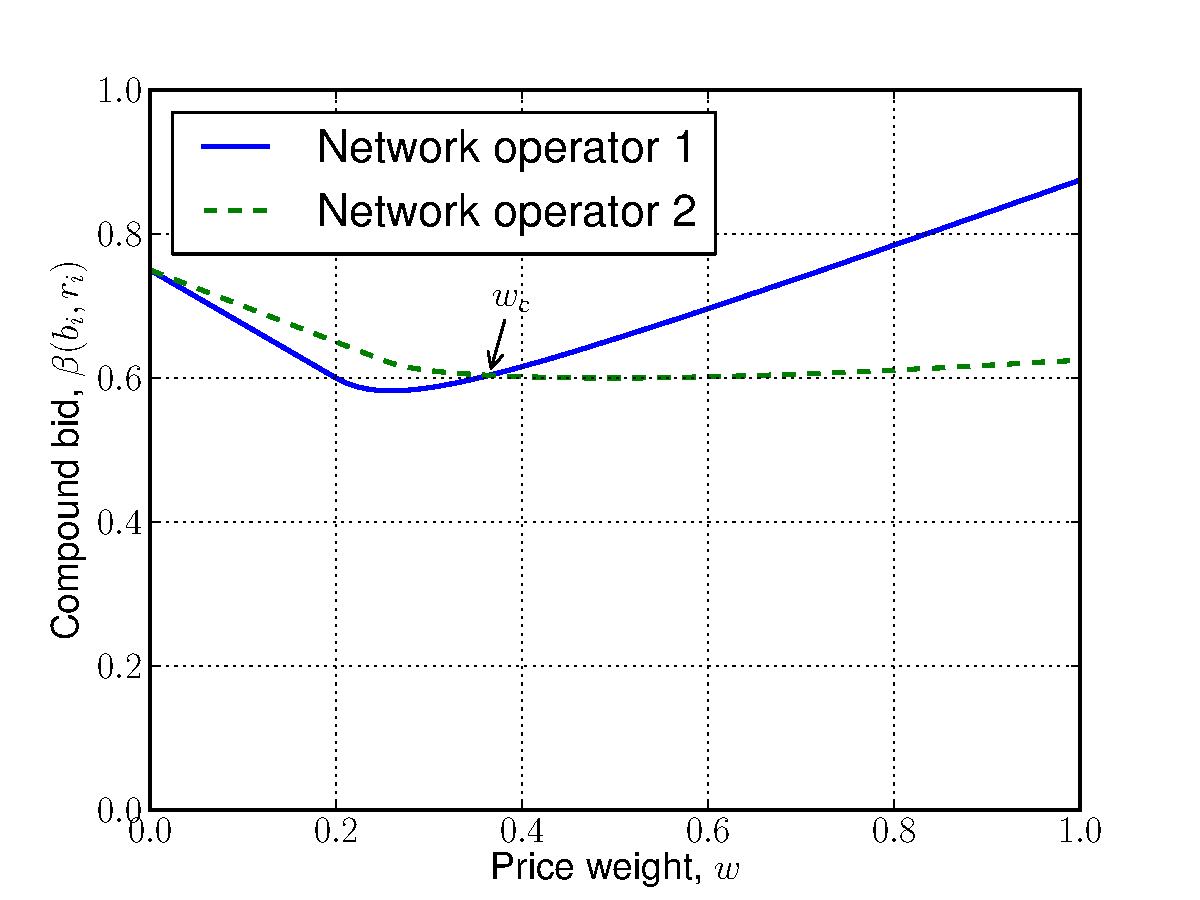
\includegraphics[width=\figsize]{Indirect/Figures/bids_restricted}
  \caption{Compound bid plotted against the price weight}
  \label{fig:bids_restricted_indirect}
  \vspace{10mm}
  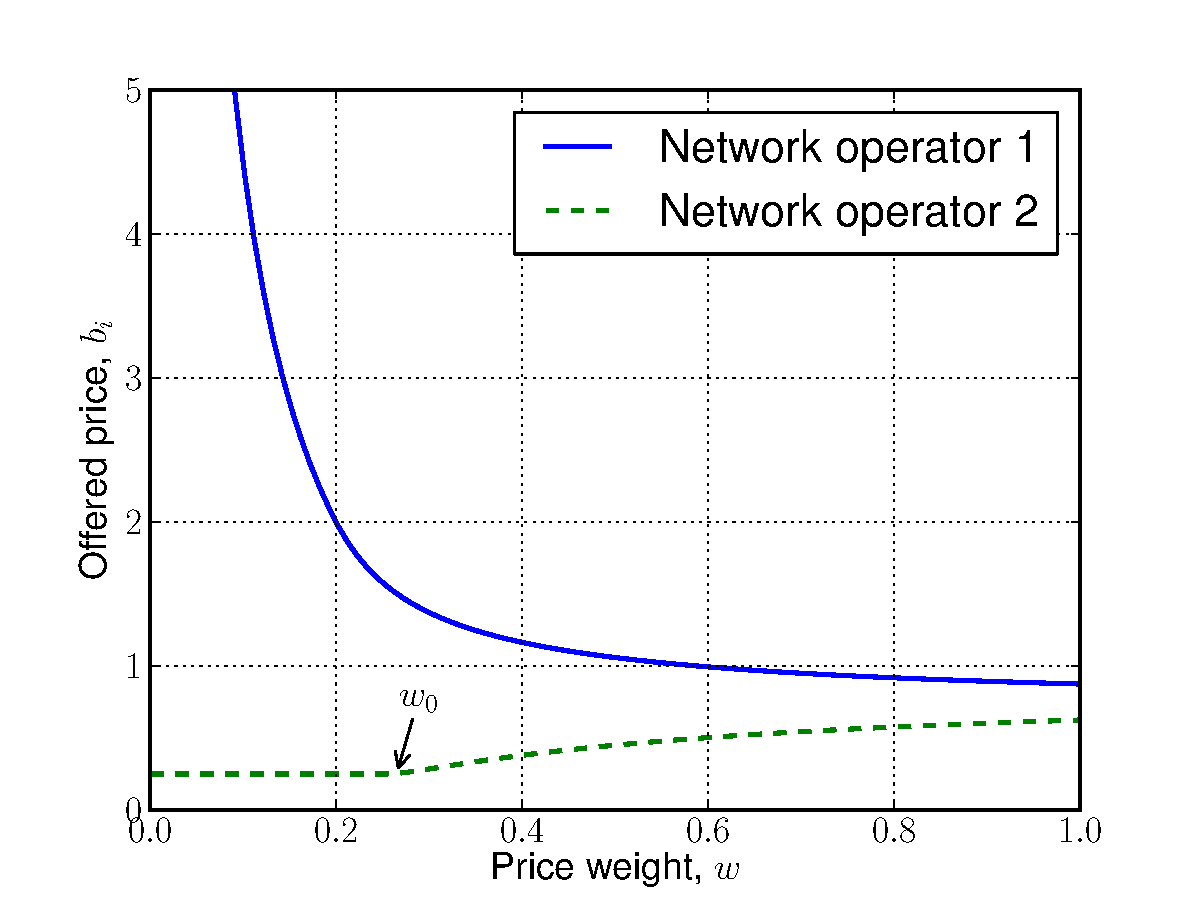
\includegraphics[width=\figsize]{Indirect/Figures/prices_restricted}
  \caption{Offered prices (bids) plotted against the price weight}
  \label{fig:prices_restricted_indirect}
\end{figure}

The result of the steps described above is the tabulation of the costs-hat and their corresponding equilibrium bids-hat for a particular price weight $w$, and reputation ratings $r_1$ and $r_2$ for both network operators, in the ranges $[\underline{\hat{c}}_1, \bar{\hat{c}}_1]$ for network operator 1 and $[\underline{\hat{c}}_2, \bar{\hat{c}}_2]$ for network operator 2.

Denote by
\begin{equation}
  \label{eq:equi_bidding_str_1_indirect}
  \hat{b}_1(\hat{c}_1) = \hat{b}_1 \quad\textrm{for all } \hat{c}_1\in[\underline{\hat{c}}_1, \bar{\hat{c}}_1],
\end{equation}
and
\begin{equation}
  \label{eq:equi_bidding_str_2_indirect}
  \hat{b}_2(\hat{c}_2) = \hat{b}_2 \quad\textrm{for all } \hat{c}_2\in[\underline{\hat{c}}_2, \bar{\hat{c}}_2]
\end{equation}
the resultant equilibrium bidding strategy functions. The problem can be transformed back into the original domain by substituting Equations~\eqref{eq:b_hat_indirect}~and~\eqref{eq:cost_hat_indirect} into Equations~\eqref{eq:equi_bidding_str_1_indirect}~and~\eqref{eq:equi_bidding_str_2_indirect}; that is,
\begin{equation}
  \hat{b}_1(\hat{c}_1) = \hat{b}_1 \iff b_1 = \displaystyle\frac{\hat{b}_1(wc_1 + (1-w)r_1) - (1-w)r_1}{w}
\end{equation}
for all $c_1\in[0,1]$, and
\begin{equation}
  \hat{b}_2(\hat{c}_2) = \hat{b}_2 \iff b_2 = \displaystyle\frac{\hat{b}_2(wc_2 + (1-w)r_2) - (1-w)r_2}{w}
\end{equation}
for all $c_2\in[0,1]$.
Keeping costs and reputation ratings fixed, one can then estimate the equilibrium bidding strategy functions with respect to the price weights by sliding the value of $w\in(0,1)$.

\begin{table}[t]
  \caption{An exemplary set of cost-reputation pairs of two network operators}
  \vspace{0.5cm}
  \begin{tabular*}{0.5\columnwidth}[L]{@{\extracolsep{\fill}}r c c}
    \hlx{vhv}
    & \textbf{Cost}, $c_i$ & \textbf{Reputation rating}, $r_i$\\
    \hlx{vhv}
    \textbf{Network operator 1} & $0.75$ & $0.25$\\
    \textbf{Network operator 2} & $0.25$ & $0.75$\\
    \hlx{vhs}
  \end{tabular*}
  \label{tab:example_restricted_indirect}
\end{table}

By way of example, the equilibrium bidding strategy functions were estimated for the set of cost-reputation pairs depicted in Table~\ref{tab:example_restricted_indirect}. Figure~\ref{fig:bids_restricted_indirect} shows the value of the compound bid, $\beta(b_i,r_i)$, for different values of $w$ for both network operators, while Figure~\ref{fig:prices_restricted_indirect} depicts the value of the monetary bid (or offered price), $b_i$, for different values of $w$ for both network operators. The numerical data in Table~\ref{tab:example_restricted_indirect} suggests that network operator 2 should be the winner for the values of $w\rightarrow 1$ since network operator 2's cost is strictly lower than that of their opponent's. On the other hand, network operator 1 should be winner for the values of $w\rightarrow 0$ since network operator 1's reputation rating is strictly lower than that of their opponent's (which implies that network operator 1's reputation is in fact strictly higher than that of their opponent's). This prediction agrees with the numerical output shown in Figure~\ref{fig:bids_restricted_indirect}. Let $w_c$ denote the value of $w$ for which an intersection between the compound bids of both network operators occurs (if it exists). In Figure~\ref{fig:bids_restricted_indirect}, $w_c\approx 0.365$. Hence, network operator 2 wins the auction for the values of $w_c < w < 1$, while network operator 1 for the values of $0 < w < w_c$.

Note, furthermore, that since it was explicitly required for the network operators to bid their own costs when their probability of winning is zero, the monetary bid of network operator 2 is capped at their cost, $b_2 = 0.25$, for the values of $0 < w \le w_0$ where $w_0\approx 0.265$ (see Figure~\ref{fig:prices_restricted_indirect}). In the same range of $w$, as $w$ decreases, network operator 1's bid increases in an exponential-like fashion, to finally culminate in $b_1\to\infty$ at $w=0$ in accordance with Proposition~\ref{prop:special_case_w_0_direct}. As $w\to 1$, on the other hand, the monetary bids of both network operators tend to the values specified in Proposition~\ref{prop:special_case_w_1_direct}, that is, $b_1=0.875$ and $b_2=0.625$, to finally attain those values at $w=1$.

Having derived the equilibrium bidding strategy functions, it is possible to examine the expected prices the subscriber will have to pay for different values of the price weight given the reputation ratings of the network operators. This is examined next.

\subsection{Subscriber's Perspective: Expected Prices} % (fold)
\label{sub:subscriber_s_perspective_expected_prices_indirect}
Suppose there are two network operators, and costs are uniformly distributed over the interval $[0,1]$. \annotate{C5.7}{The expected price is equivalent to the expected value of the winning bid; that is,}
\begin{equation}
  \label{eq:exp_price_def_indirect}
  E[p](w,r_1,r_2) = E[b_i \:\vert\: \arg\min_{i\in \{1,2\}}\beta(w,b_i,r_i)],
\end{equation}
where $b_i$ is the equilibrium bid, and $\beta(w,b_i,r_i) = \beta(b_i,r_i)$ evaluated for a particular value of $w$ for all $i\in \{1,2\}$.

If both network operators have equal reputation ratings, $r = r_1 = r_2$ say, then Corollary~\ref{cor:special_case_r_i_r_j_direct} holds for all $w\in [0,1]$. Therefore, regardless of the choice of the price weight, the subscriber expects to pay the price of
\begin{equation}
  \label{eq:exp_price_at_w_1_indirect}
  E[p^*] = E[p](w,r,r) = E\left[\min_{i\in \{1,2\}}\frac{1+c_i}{2}\right] \quad\textrm{for all } w\in [0,1],
\end{equation}
which is equivalent to Equation~\eqref{eq:standard_fpa_direct} evaluated at $n=2$. In particular, for costs, $c_i$, uniformly distributed over the interval $[0,1]$, $E[p^*] = \frac{2}{3}$.

If, on the other hand, both network operators are characterised by different reputation ratings, then an analytical derivation of the expected prices for each value of the price weight given a pair of reputation ratings is cumbersome. This is due to the fact that network operators bid according to a pair of inverse equilibrium bidding functions specified in Proposition~\ref{prop:equilibrium_restricted_indirect}, which are not easily invertible. Hence, numerical method is used to estimate average (sample mean) prices for selected values of the price weight given a pair of reputation ratings.

\begin{figure}[p!]
  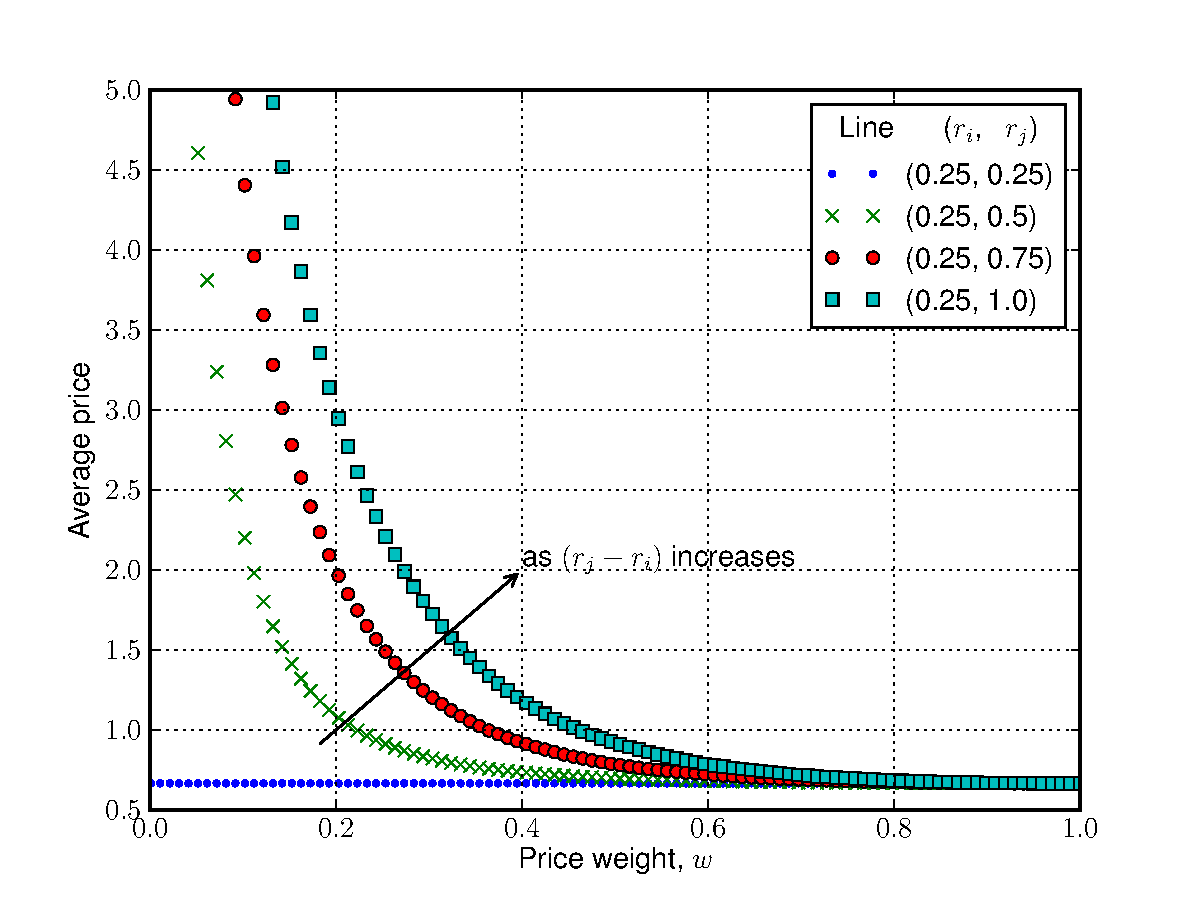
\includegraphics[width=\figsize]{Indirect/Figures/expected_prices}
  \caption{Average prices plotted against the price weight for different pairs of reputation ratings}
  \label{fig:expected_prices_indirect}
  \vspace{10mm}
  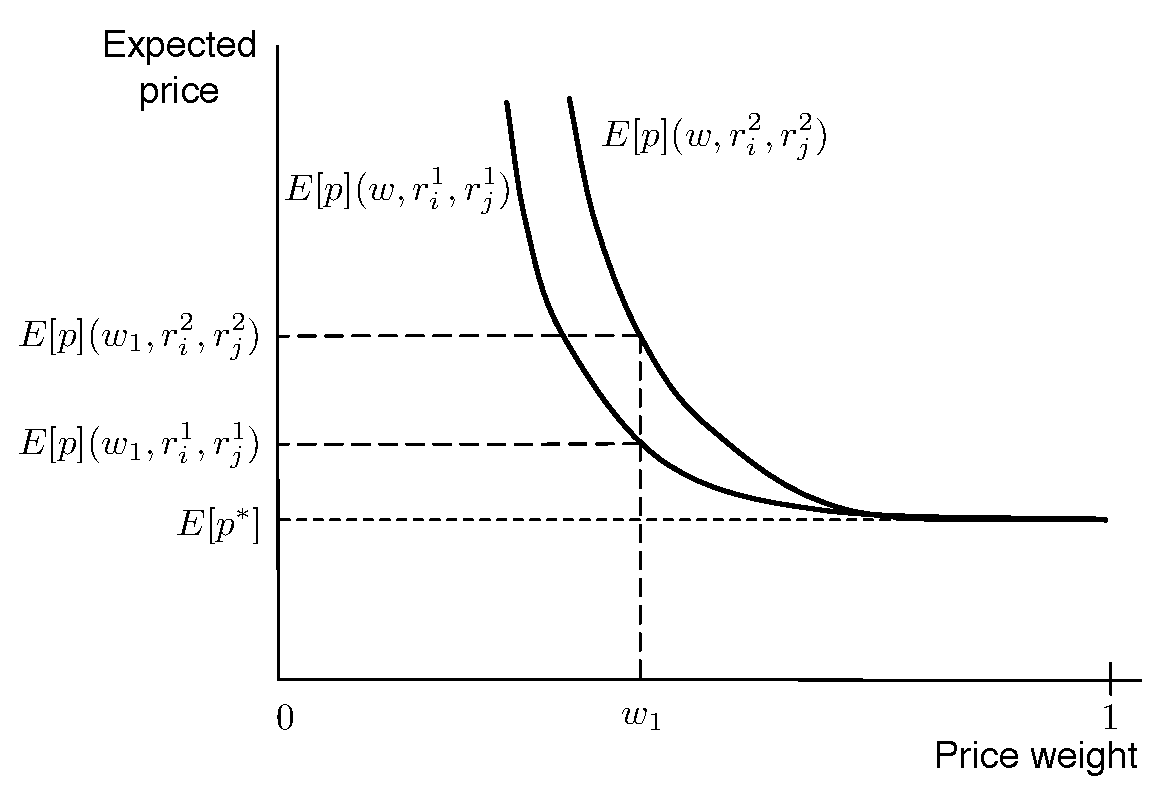
\includegraphics[width=\figsize]{Indirect/Figures/expected_prices_sensitivity}
  \caption{Sensitivity of the price weight to the expected prices}
  \label{fig:expected_prices_sensitivity_indirect}
\end{figure}

To this end, for any given pair of reputation ratings, the costs are pseudo-randomly drawn from the uniform distribution over the discretised interval $[0,1]$. For each selected price weight, the average price is averaged over 10,000 i.i.d.~observations. The Strong Law of Large Numbers implies that as the number of observations tends to infinity, the average (sample mean) of the observations approaches the real mean of the distribution of the r.v.~in question (see Section~\ref{sub:strong_law_of_large_numbers_notation}, Appendix~\ref{cha:notation} for the definition of the Strong Law of Large Numbers). \annotate{C5.8}{Furthermore, it was empirically established that averaging over more than 10,000 observations does not drastically improve the results; that is, the already narrow 95\% confidence intervals do not get narrower as the number of observations increases beyond 10,000. In other words, 10,000 is large enough a sample size, and therefore, an average of 10,000 observations of the price for each selected price weight should provide a reasonable approximation of the expected price for that price weight.} Without loss of generality, suppose further that $r_1 \le r_2$. Figure~\ref{fig:expected_prices_indirect} shows the result of the estimation for four pairs of reputation ratings: $(r_1, r_2) = (0.25, 0.25)$, $(0.25, 0.5)$, $(0.25, 0.75)$, and $(0.25, 1.0)$.

It can be observed that regardless of the values of the reputation ratings, the expected prices, $E[p](w,r_1,r_2)$, are bounded from below by $E[p^*]$ for each price weight; this is depicted in Figure~\ref{fig:expected_prices_indirect}. Hence, it can be concluded that regardless of the values of the reputation ratings, the lowest expected price is achieved for $w=1$, and will not decrease as $w$ decreases; in fact, it can only either increase or remain constant.

Furthermore, as the difference $(r_2-r_1)$ increases, the expected prices, $E[p](w,r_1,r_2)$, increase as the price weight decreases; this is depicted in Figure~\ref{fig:expected_prices_indirect}. Therefore, it can be hypothesised that the smaller the difference $(r_2-r_1)$, the less (expected) price sensitive the price weight; \annotate{C5.9}{that is, for any $w_1\in[0,1]$, if $(r^{(2)}_2-r^{(2)}_1) > (r^{(1)}_2-r^{(1)}_1)$ for all $r^{(1)}_1,r^{(1)}_2,r^{(2)}_1,r^{(2)}_2\in [0,1]$, then $E[p](w_1,r^{(2)}_1,r^{(2)}_2) \ge E[p](w_1,r^{(1)}_1,r^{(1)}_2)$ (see Figure~\ref{fig:expected_prices_sensitivity_indirect}).} \annotate{C5.10}{In other words, for any expected price, as the difference $(r_2-r_1)$ between the reputation ratings of the network operators increases, the price weight has to increase (or remain constant) in order to keep the expected price fixed. This observation carries very serious implications on the operation of the DMP, as the subscriber is effectively given the ability to influence the expected prices by an appropriate choice of the price weight. To illustrate, suppose there are 2 network operators characterised by reputation ratings $(r_1, r_2)$. Suppose further that the subscriber paid the price of $p_1$ at some point in the past for some type of service, and they request the same service again. Therefore, in order to pay the expected price of at most $p_1$, the subscriber solves
\begin{equation}
  p_1 \ge E[p_1](w, r_1, r_2)
\end{equation}
for the price weight $w$. In this way, the subscriber is guaranteed the expected price of at most $p_1$.}
% subsection subscriber_s_perspective_expected_prices_in_restricted_case (end)

As already mentioned in the previous section, the bidding problem does not possess a closed-form solution in the case of more than two network operators. However, it is possible to approximate the solution numerically, as it will be discussed in the next section. It should further be noted that the equilibrium bidding strategies derived in this section will be used to verify the correctness of the numerical methods presented in the next section.
% section restricted_case_n_2_indirect (end)

\section{Numerical Analysis} % (fold)
\label{sec:numerical_analysis_indirect}
Precisely because the system of ODEs~\eqref{eq:foc_ode_indirect} together with the lower and upper boundary conditions~\eqref{eq:foc_ode_lower_boundary_indirect}~and~\eqref{eq:foc_ode_upper_boundary_indirect} does not possess any known closed-form solution in a generic setting, and especially when $n>2$, there exists a considerable research base studying methods for numerical approximation of the solution to the system of ODEs in question. See Hubbard and Paarsch~\cite{HubbardPaarsch2011} for an excellent overview of the subject.

The literature is mostly concerned with asymmetric first-price auctions in which the bidders are characterised by different probability distributions sharing a common support; that is, $F_i(x)\neq F_j(x)$ for at least one $i\in N$ such that $i\neq j, j\in N$, and for all $x\in [\underline{\hat{c}}, \bar{\hat{c}}]$ where $[\underline{\hat{c}}, \bar{\hat{c}}] = [\underline{\hat{c}}_i, \bar{\hat{c}}_i]$ for all $i\in N$. This is not true in this case. Therefore, the methods described in Hubbard and Paarsch~\cite{HubbardPaarsch2011} have to be adapted before they can be applied to the problem under investigation here.

\annotate{C5.21}{Firstly, it should be noted that there exist many methods of numerically approximating the solutions to a system of (ordinary or partial) differential equations; but, finite-difference methods, such as Euler or Runge-Kutta methods, are particularly well suited to solving systems of ODEs~\cite{Butcher2008,GriffithsHigham2010}. In the problem at hand, since the system of ODEs satisfies the Lipschitz condition of continuity at the lower boundary condition $\underline{\hat{b}}$, if $\underline{\hat{b}}$ was known, standard finite-difference methods would apply~\cite{Bajari2001a} (see Section~\ref{sub:lipschitz_condition_notation}, Appendix~\ref{cha:notation} for the definition of Lipschitz condition). However, this is not true in both scenarios, the one considered in the literature and the one at hand: the common lower bound on bids, $\underline{\hat{b}}$, is unknown \emph{a priori} \cite{HubbardPaarsch2011}}. On the other hand, since the common upper bound on bids, $\bar{\hat{b}}$, is known \emph{a priori}, it would seem that the finite-difference methods could be applied to the system of ODEs in Equation~\eqref{eq:foc_ode_indirect} with the upper bound on bids as a starting point (the so-called \emph{terminal value problem} as opposed to the more common \emph{initial value problem}). As shown by Hubbard and Paarsch~\cite{HubbardPaarsch2011}, the system does not satisfy the Lipschitz condition as the solution approaches the upper bound on bids, $\bar{\hat{b}}$. Therefore, much of the theory of ordinary differential equations no longer applies. In practice, this effectively means that the numerical solution obtained using a finite-difference method applied to the terminal value problem will quickly diverge. This is depicted in Figure~\ref{fig:lipschitz_indirect}. In this scenario, there are 2 network operators characterised by reputation ratings $r_1 = 0.25$ and $r_2 = 0.75$, and the price weight is set to $w=0.5$. The $4^{\textrm{th}}$-order backwards Runge-Kutta method is used to numerically solve the terminal value problem. It is clear in the figure that the numerical solution tracks the analytical equilibrium path only for $\hat{b}\in [0.72, 0.75]$, while it diverges for all the remaining values of bid-hat, $\hat{b}\in [0.515625, 0.72)$. Note, further, that after the solution diverges, it never recovers rendering the approximation useless.

\begin{figure}[t]
  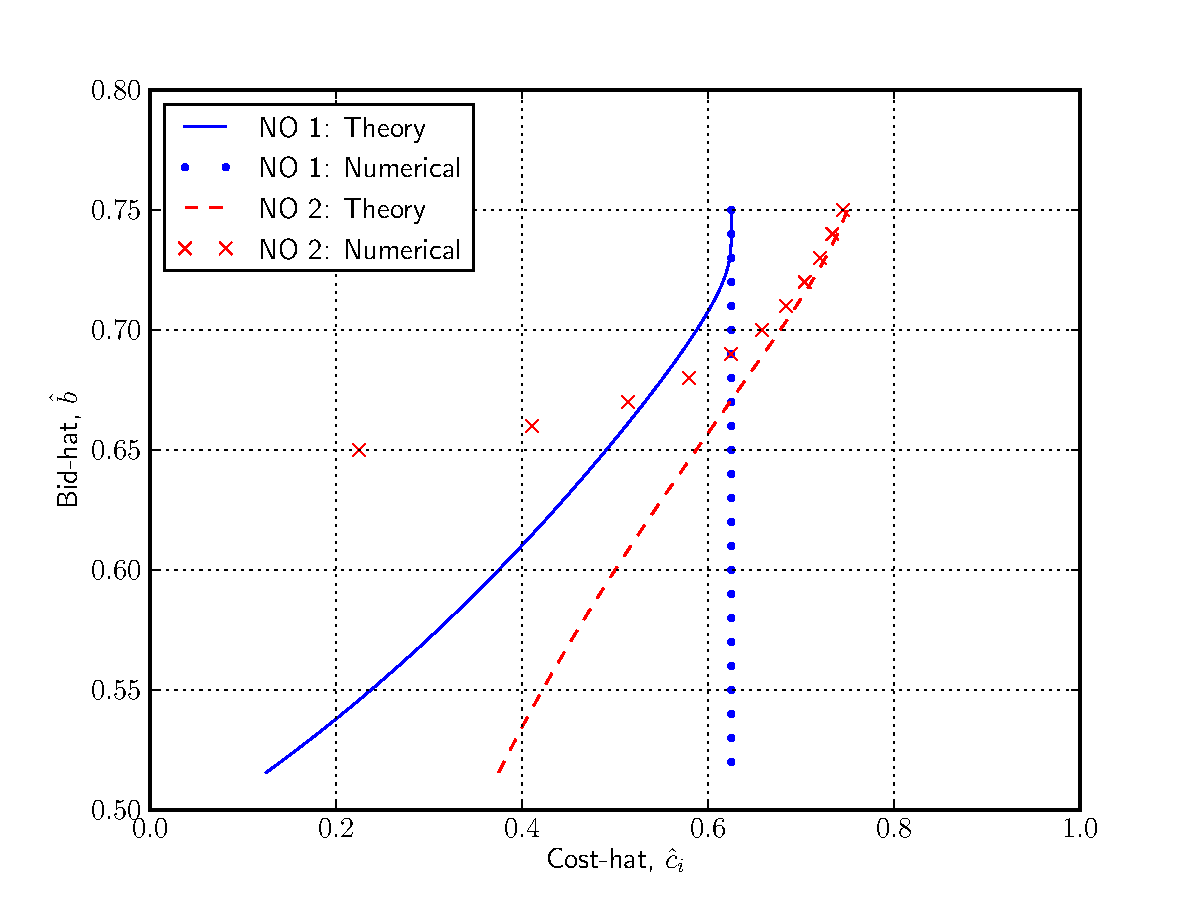
\includegraphics[width=\figsize]{Indirect/Figures/lipschitz}
  \caption{Violation of Lipschitz condition leads to divergent numerical solution}
  \label{fig:lipschitz_indirect}
\end{figure}

In this section, two numerical algorithms are considered which overcome the aforementioned problem: the forward shooting method (FSM), and the polynomial projection method (PPM), both of which were first proposed by Bajari~\cite{Bajari2001a}. \annotate{C5.22}{The problem naturally fits into the framework of the FSM method since, as discussed in the previous paragraph, if the lower boundary condition, $\underline{\hat{b}}$, was known, standard finite-difference methods could be used to a great success in finding a numerical solution to the system of ODEs. As demonstrated in the subsequent section, the FSM method tries iteratively to guess the lower boundary condition, and for each guess, it then uses finite-difference methods to numerically solve the system of ODEs. Furthermore, the thesis focuses on the FSM and PPM methods since they are the simplest out of all of the available algorithms described in Hubbard and Parsch~\cite{HubbardPaarsch2011}, and hence, they pose the least technical difficulties when adapting to the problem at hand, and yet yield numerical results of acceptable quality to permit conlusions to be drawn.} To this end, let costs, $c_i$, be drawn from a uniform distribution for all network operators as in Section~\ref{sec:restricted_case_n_2_indirect}. Again, this implies that the distribution of costs-hats, $\hat{c}_i$, is uniform with supports $[\underline{\hat{c}}_i, \bar{\hat{c}}_i] = [(1-w)r_i, (1-w)r_i + w]$ for all $i\in N$. The discussion concentrates only on cases in which $J=N$; that is, $\underline{\hat{c}}_i < \bar{\hat{b}}$ for all $i\in N$. In particular, it is required $w\in\left(0.5, 1\right)$ which immediately implies $\underline{\hat{c}}_i < \bar{\hat{b}}$ for all $i\in N$. To see this, without loss of generality, suppose $r_1\leq\cdots\leq r_n$ with at least one inequality strict. Since $\bar{\hat{b}}\in[\bar{\hat{c}}_1, \bar{\hat{c}}_2]$ by Definition~\ref{def:upper_bound_bids_indirect}, and in particular, if $\underline{\hat{c}}_n < \bar{\hat{c}}_1$, then $\underline{\hat{c}}_n < \bar{\hat{b}}$. Thus, it is required $\underline{\hat{c}}_n = (1-w)r_n < (1-w)r_1 + w = \bar{\hat{c}}_1$. This is equivalent to $1 - \frac{1}{1+r_n-r_1} < w$. Since $(r_n - r_1)\in (0, 1]$, then $1 - \frac{1}{1+r_n-r_1} \in (0,0.5]$. Therefore, if $0.5 < w$, then $1 - \frac{1}{1+r_n-r_1} < w$ for all $(r_n-r_1)\in (0,1]$.

Furthermore, note that assumption 3 in Assumptions~\ref{ass:assumptions_generic_indirect} is satisfied even if there exists two or more network operators characterised by the lowest reputation rating. To see this, let, without loss of generality, network operators 1 and 2 be characterised by the lowest reputation rating. Then, $\bar{\hat{c}}_1 = \bar{\hat{c}}_2$. Recall that $\bar{\hat{b}}\in [\bar{\hat{c}}_1, \bar{\hat{c}}_2]$ by Definition~\ref{def:upper_bound_bids_indirect}. Thus, $\bar{\hat{b}} = \bar{\hat{c}}_1$. For assumption 3 in Assumptions~\ref{ass:assumptions_generic_indirect} not to hold, it is required $\bar{\hat{b}} = \bar{\hat{c}}_1 \leq \underline{\hat{c}}_i$ for any $i\in N$ and any $\delta>0$. But this means network operator $i$ is not a feasible bidder; that is, $i\not\in J$ by Definition~\ref{def:feasible_bidders_indirect}. A contradiction since it was assumed $J = N$. Now, let $\delta = \bar{\hat{b}} - \underline{\hat{c}}_n > 0$ where $n = |N|$; that is, $r_1\leq r_n$. Then,
\begin{equation}
(\bar{\hat{b}}-\delta, \bar{\hat{b}})\cap (\underline{\hat{c}}_i, \bar{\hat{c}}_i) = (\underline{\hat{c}}_n, \bar{\hat{b}})\cap (\underline{\hat{c}}_i, \bar{\hat{c}}_i) = (\underline{\hat{c}}_n, \bar{\hat{b}})
\end{equation}
for all $i\in N$. The resulting set is convex, and since $(\underline{\hat{c}}_n, \bar{\hat{b}})\subset [\underline{\hat{c}}_i, \bar{\hat{c}}_i]$ for all $i\in N$, this implies that $F_i$ is strictly log-concave over $(\bar{\hat{b}}-\delta, \bar{\hat{b}})\cap (\underline{\hat{c}}_i, \bar{\hat{c}}_i)$ for all $i\in N$.

Finally, the discussion will concentrate on cases such that
\begin{equation}
  \label{eq:simplification_foc_ode_indirect}
  \underline{\hat{c}}_i \leq \hat{c}(\underline{\hat{b}}) \quad\textrm{for all } i\in N.
\end{equation}
\annotate{C5.5}{This requirement simplifies the problem so that it is numerically tractable using existing numerical methods.} More specifically, it reduces the lower boundary condition in Equation~\eqref{eq:foc_ode_lower_boundary_indirect} to
\begin{equation}
  \label{eq:foc_ode_lower_boundary_reduced_indirect}
  \hat{c}_i(\underline{\hat{b}}) = \underline{\hat{c}}_i \quad\textrm{for all } i\in N.
\end{equation}
\annotate{C5.18}{The ultimate aim of the numerical analysis is to obtain a numerical approximation to the equilibrium bidding strategies for all bidding scenarios that involve feasible bidders (cf.~Definition~\ref{def:feasible_bidders_indirect}). However, as shown below, the assumption~\eqref{eq:simplification_foc_ode_indirect} restricts the choice of the price weight and the reputation ratings to a subset of all possible bidding scenarios involving feasible bidders.} Without this assumption, as explained by Lebrun~\cite{Lebrun2006}, there might exist $i$ such that
\begin{equation}
  \hat{c}(\underline{\hat{b}}) < \underline{\hat{c}}_i < \bar{\hat{b}}
\end{equation}
which forces the bid function $\hat{b}_i$ to be extended to the interval $[\hat{c}(\underline{\hat{b}}), \bar{\hat{b}}]$, which is strictly larger than the actual support, truncated at $\bar{\hat{b}}$, $[\underline{\hat{c}}_i, \bar{\hat{b}}]$ of network operator $i$'s cost. This result is somewhat confusing since even though $F_i(\hat{c}_i) = 0$ for all $\hat{c}_i\in [\hat{c}(\underline{\hat{b}}), \underline{\hat{c}}_i]$, $\hat{b}_i(\hat{c}_i)$ is still network operator $i$'s best response for all $\hat{c}_i\in [\hat{c}(\underline{\hat{b}}), \underline{\hat{c}}_i]$. The main difficulty when considering such cases stems from the fact that for all $i\in I$, where $I = \left\{i\in N \:\middle\vert\: \hat{c}(\underline{\hat{b}}) < \underline{\hat{c}}_i < \bar{\hat{b}} \right\}$, the system of ODEs in Equation~\eqref{eq:foc_ode_indirect} reduces to
\begin{equation}
  \label{eq:foc_reduced_indirect}
  0 = \frac{1}{n-1}\sum_{k=1}^{n}\frac{1}{b - \hat{c}_k(b)} - \frac{1}{b - \hat{c}_i(b)}.
\end{equation}
As further explained by Lebrun~\cite{Lebrun2006}, the (inverse) equilibrium bidding functions are then determined by
\begin{equation}
  \label{eq:foc_ode_reduced_indirect}
  \frac{d}{db}\hat{c}_j(b) = \frac{1 - F_j(\hat{c}_j(b))}{f_j(\hat{c}_j(b))} \left[ \frac{1}{k(\underline{\hat{b}}) - 1}\sum_{\substack{k\in N\\ k\not\in I}}\frac{1}{b - \hat{c}_k(b)} - \frac{1}{b - \hat{c}_j(b)}\right]
\end{equation}
for network operators $j\in N, j\not\in I$, and by the system in Equation~\eqref{eq:foc_reduced_indirect} for network operators $i\in I$. Both systems are combined for all $b > \underline{\hat{b}}$ until the common function $\hat{c}_i$, $i\in I$, takes as its value the smallest lower extremity strictly smaller than $\hat{c}(\underline{\hat{b}})$. At the bid where this next smallest lower extremity is reached, the functions $\hat{c}_i$ of the network operators with this lower extremity of their supports are added to the system in Equation~\eqref{eq:foc_ode_reduced_indirect}. This process is repeated until $\hat{c}_i$ for all $i\in N$ are included in~\eqref{eq:foc_ode_reduced_indirect}. This procedure is not easily accommodated by any of the numerical methods described in the literature; hence, the assumption
\begin{equation}
  \underline{\hat{c}}_i \leq \hat{c}(\underline{\hat{b}}) \quad\textrm{for all } i\in N.
\end{equation}
Note, however, that this assumption cannot be enforced \emph{a priori} since $\underline{\hat{b}}$ is unknown. The (approximate) probability of enforcing this condition can be maximised by reasoning as follows. Without loss of generality, suppose $r_1\leq\cdots\leq r_n$ with at least one inequality strict. If $k(\underline{\hat{b}})=n$, then, by Definition~\ref{def:lower_bound_bids_indirect}, $\underline{\hat{c}}_n\leq \hat{c}(\underline{\hat{b}})$ and $\underline{\hat{c}}_n < \underline{\hat{b}}$. Furthermore, since $\underline{\hat{b}}\in (\underline{\hat{c}}_2, \bar{\hat{b}})$, then as the distance $(\underline{\hat{c}}_n-\underline{\hat{c}}_2)\to 0$, $k(\underline{\hat{b}})\to n$. Thus, the probability that $\underline{\hat{b}}\in (\underline{\hat{c}}_n, \bar{\hat{b}})$ (assuming $\underline{\hat{b}}$ is distributed uniformly over $(\underline{\hat{c}}_2, \bar{\hat{b}})$) can be quantified as follows
\begin{equation}
  P\left\{ \underline{\hat{b}}\in (\underline{\hat{c}}_n, \bar{\hat{b}}) \right\} = 1 - P\left\{\underline{\hat{b}}\in(\underline{\hat{c}}_2, \underline{\hat{c}}_n)\right\} = 1 - \frac{\underline{\hat{c}}_n - \underline{\hat{c}}_2}{\bar{\hat{b}}-\underline{\hat{c}}_2} = \frac{\bar{\hat{b}} - \underline{\hat{c}}_n}{\bar{\hat{b}} - \underline{\hat{c}}_2}.
\end{equation}
\annotate{C5.4}{For example}, for the probability of at least $0.9$, it is required
\begin{equation}
  \frac{\bar{\hat{b}} - \underline{\hat{c}}_n}{\bar{\hat{b}} - \underline{\hat{c}}_2} \geq 0.9 \iff \bar{\hat{b}}\geq 10\underline{\hat{c}}_n - 9\underline{\hat{c}}_2.
\end{equation}
Since $\bar{\hat{c}}_1\leq \bar{\hat{b}}$ by Definition~\ref{def:upper_bound_bids_indirect}, it follows that
\begin{equation}
  \bar{\hat{c}}_1 \geq 10\underline{\hat{c}}_n - 9\underline{\hat{c}}_2 \iff w \geq 1 - \frac{1}{10r_n - 9r_2 - r_1 + 1}.
\end{equation}
Note that, since it was assumed $r_1\leq\cdots\leq r_n$ with at least one inequality strict, the denominator is always strictly greater than $1$ ($10r_n - 9r_2-r_1+1 > 1$), hence guaranteeing the right-hand side of the inequality to be smaller than $1$.

To conclude, the rest of this section will concentrate on cases such that
\begin{equation}
  w \in (0.5, 1) \quad\textrm{and}\quad w \geq 1 - \frac{1}{10r_n - 9r_2 - r_1 + 1}
\end{equation}
for all $r_1,r_2,r_n\in [0,1]$ such that $r_1\leq\cdots\leq r_n$ with at least one inequality strict.

In what follows, firstly the inner workings of the FSM and PPM methods are outlined, and then the numerically approximated equilibrium bidding strategies are presented for two bidding scenarios generated using both algorithms. \annotate{C5.19}{In both cases, it is assumed without loss of generality that network operator 1 is characterised by the lowest reputation rating, network operator 2 by the second lowest, and so on. Hence, $\underline{\hat{c}}_1\leq \underline{\hat{c}}_2\leq \underline{\hat{c}}_i$ and $\bar{\hat{c}}_1\leq \bar{\hat{c}}_2\leq \bar{\hat{c}}_i$ for all $i\geq 2$.}

\subsection{Forward Shooting Method} % (fold)
\label{sub:forward_shooting_method_indirect}
The idea behind the FSM is to find the best approximation of the lower bound on bids, $\underline{\hat{b}}'$ say, by successively picking a value from the feasible interval $(\underline{\hat{c}}_2, \bar{\hat{b}})$, and verifying whether a numerical solution to the initial value problem
\begin{equation}
  \label{eq:fsm_initial_value_problem_indirect}
  \begin{array}{ll}
    \displaystyle\frac{d}{db}\hat{c}_i(b) &= \displaystyle\frac{1 - F_i(\hat{c}_i(b))}{f_i(\hat{c}_i(b))}\left[ \frac{1}{n-1}\sum_{k=1}^n\frac{1}{b - \hat{c}_k(b)} - \frac{1}{b - \hat{c}_i(b)} \right] \\[2ex]
    \hat{c}_i(\underline{\hat{b}}') &= \underline{\hat{c}}_i
  \end{array}
\end{equation}
\annotate{C5.14}{for all $i\in N$ satisfies the following three conditions: 1) it is a function mapping $[\underline{\hat{b}}', \bar{\hat{b}}]$ into $[\underline{\hat{c}}_i, \bar{\hat{c}}_i]$, that is,
\begin{equation}
  \label{eq:fsm_condition_1_indirect}
  s_i: [\underline{\hat{b}}', \bar{\hat{b}}]\to [\underline{\hat{c}}_i, \bar{\hat{c}}_i];
\end{equation}
2) it is monotonically increasing everywhere except possibly at $\bar{\hat{b}}$, that is,
\begin{equation}
  \label{eq:fsm_condition_2_indirect}
  b_1 < b_2\implies s_i(b_1) < s_i(b_2) \textrm{ for all }b_1,b_2\in [\underline{\hat{b}}', \bar{\hat{b}});
\end{equation}
and 3) each function value is strictly lower than its argument except possibly at $\bar{\hat{b}}$, that is,
\begin{equation}
  \label{eq:fsm_condition_3_indirect}
  s_i(b) < b \textrm{ for all }b\in [\underline{\hat{b}}', \bar{\hat{b}}).
\end{equation}}

This specification of the problem is a modified version of the First Algorithm in Bajari~\cite{Bajari2001a} (cf.~Section~3.3 in~\cite{Bajari2001a}) that accommodates for different lower and upper extremities in the supports of bidders' costs.

\begin{algorithm}
\caption{Forward shooting method}
\label{alg:forward_shooting_method_indirect}
\begin{algorithmic}[1]
\Require{$\epsilon\in (0, \bar{\hat{b}} - \underline{\hat{c}}_2); low, high\in [\underline{\hat{c}}_2, \bar{\hat{b}}]$ such that $low\leq high$}
\Ensure{Approximation to $\underline{\hat{b}}$}
  \Statex
  \Let{$low$}{$\underline{\hat{c}}_2$}
  \Let{$high$}{$\bar{\hat{b}}$}
  \Statex
  \While{$high-low > \epsilon$}
    \Let{$guess$}{$0.5\cdot(low + high)$}
    \Let{$bids$}{$[guess, \bar{\hat{b}})$}
    \Let{$(costs_1,\dotsc,costs_n)$}{solve~\eqref{eq:fsm_initial_value_problem_indirect} with initial value $\underline{\hat{b}}' = guess$}
    \StatexIndent[7.5]{evaluated at points $b\in bids$}
    \If{$(bids,costs_i)$ satisfies~\eqref{eq:fsm_condition_1_indirect}, \eqref{eq:fsm_condition_2_indirect} and \eqref{eq:fsm_condition_3_indirect} for all $i\gets 1$ to $n$}
      \Let{$high$}{$guess$}
    \Else
      \Let{$low$}{$guess$}
    \EndIf
  \EndWhile
  \Statex
  \Let{$\underline{\hat{b}}'$}{$0.5\cdot(low + high)$}
\end{algorithmic}
\end{algorithm}

The pseudo-code for the FSM is depicted in listing Algorithm~\ref{alg:forward_shooting_method_indirect}. For any given tolerance, $\epsilon\in\left(0, \bar{\hat{b}} - \underline{\hat{c}}_2\right)$, the algorithm aims at finding the interval $LH=[low, high]\subseteq [\underline{\hat{c}}_2, \bar{\hat{b}}]$ such that (approximately) $\underline{\hat{b}}\in LH$ and $high-low < \epsilon$. The approximation to the lower bound on bids is then found to be $\underline{\hat{b}}' = 0.5\cdot(low + high)$.

The initial guess supplied to the algorithm is the interval $[\underline{\hat{c}}_2, \bar{\hat{b}}]$. In every iteration, the guessed value for the lower bound on bids is the midpoint of the interval; that is, $guess = 0.5\cdot(low + high)$. The algorithm then uses this value as the new initial condition for the system in~\eqref{eq:fsm_initial_value_problem_indirect}. If the solution to the system lies within the set $S_i$ for all $i\in N$, then $guess$ becomes the new upper endpoint of the interval $LH$; that is, $LH = [low, guess]$. Otherwise, it becomes the new lower endpoint; that is, $LH = [guess, high]$. This procedure is repeated until the length of the interval is smaller than $\epsilon$.

In each step, the system of ODEs in~\eqref{eq:fsm_initial_value_problem_indirect} can be solved numerically using any type of finite-difference methods, such as Euler or Runge-Kutta methods. The results presented in this section were obtained using the GNU Scientific Library (GSL) implementation of the Embedded Runge-Kutta-Fehlberg (4, 5) method~\cite{GSL}.

Furthermore, in the implementation of the FSM, it was assumed that
\begin{equation}
  F_i(x) = \frac{x - \underline{\hat{c}}_i}{\bar{\hat{c}}_i - \underline{\hat{c}}_i} \quad\textrm{and}\quad f_i(x) = \frac{1}{\bar{\hat{c}}_i - \underline{\hat{c}}_i}
\end{equation}
for all $i\in N$ and $x\in\mathbb{R}$. This assumption reduces the original initial value problem in~\eqref{eq:fsm_initial_value_problem_indirect} to
\begin{equation}
  \begin{array}{ll}
    \displaystyle\frac{d}{db}\hat{c}_i(b) &= \displaystyle\left[ \bar{\hat{c}}_i - \hat{c}_i(b)\right]\cdot\left[ \frac{1}{n-1}\sum_{k=1}^n\frac{1}{b - \hat{c}_k(b)} - \frac{1}{b - \hat{c}_i(b)} \right], \\[2ex]
    \hat{c}_i(\underline{\hat{b}}') &= \underline{\hat{c}}_i,
  \end{array}
\end{equation}
and it is there mainly to avoid possible divisions by zero which are not handled properly by the GSL library. Situations like this may arise due to the nature of finite-difference methods, and the fact that the system of ODEs features a fraction
\begin{equation}
  \frac{1 - F_i(x)}{f_i(x)}
\end{equation}
which is undefined for all $x\in\mathbb{R}$ such that $x < \underline{\hat{c}}_i$ and $x > \bar{\hat{c}}_i$ (since $f_i(x) = 0$ for all $x < \underline{\hat{c}}_i$ and $x > \bar{\hat{c}}_i$). On the other hand, by enforcing this assumption, it is implicitly assumed that the algorithm always operates in the feasible region; that is,
\begin{equation}
  \hat{c}_i(b)\in [\underline{\hat{c}}_i, \bar{\hat{c}}_i] \quad\textrm{for all } i\in N \textrm{ and } b\in\left[\underline{\hat{b}}', \bar{\hat{b}}\right].
\end{equation}
This, of course, cannot be guaranteed for all choices of $\underline{\hat{b}}'$ made by the algorithm, and therefore, it might skew the final result away from the actual value of the lower bound on bids, $\underline{\hat{b}}$.
% subsection forward_shooting_method_indirect (end)

\subsection{Polynomial Projection Method} % (fold)
\label{sub:polynomial_projection_method_indirect}
The PPM method assumes that the inverse equilibrium bidding function for each network operator $i\in N$ can be approximated by a $K^{\textrm{th}}$ order polynomial of the form
\begin{equation}
  \label{eq:polynomial_cost_function_indirect}
  \hat{c}_i(b;\underline{\hat{b}}, \alpha_i) = \underline{\hat{c}}_i + \sum_{k=1}^K \alpha_{i,k}(b - \underline{\hat{b}})^k,
\end{equation}
\annotate{C5.12}{where $K\in\mathbb{N}_+$ and $K\geq 2$, and $\alpha_i = (\alpha_{i,1},\dotsc,\alpha_{i,K})^T$ is a vector of $K$ unknown polynomial coefficients such that $\alpha_i\in\mathbb{R}^{K}$.} The idea behind the method is then to employ a nonlinear optimisation technique, such as the Nelder-Mead method, to find an approximation to the lower bound on bids and the set of polynomial coefficients that best satisfy the system of ODEs~\eqref{eq:foc_ode_indirect} with lower and upper boundary conditions~\eqref{eq:foc_ode_lower_boundary_indirect} and \eqref{eq:foc_ode_upper_boundary_indirect} in the least squares sense. That is, minimise the least squares objective function
\begin{equation}
  \label{eq:least_squares_objective_function_indirect}
  H(\underline{\hat{b}}, \alpha_1,\dotsc,\alpha_n) = \sum_{i\in N}\sum_{b\in B}G_i(b; \underline{\hat{b}}, \alpha_1,\dotsc, \alpha_n)^2 + |B|\cdot\sum_{i\in N} (\bar{\hat{b}} - \hat{c}_i(\bar{\hat{b}}; \underline{\hat{b}}, \alpha_i))^2,
\end{equation}
where $B=\{\underline{\hat{b}},\dotsc,\bar{\hat{b}}\}$ is a (finite) grid of points uniformly spaced between $\underline{\hat{b}}$ and $\bar{\hat{b}}$, $|B| < \infty$ denotes the cardinality of $B$, and $G_i$ captures network operator $i$'s first-order condition for profit maximisation, and is defined as follows
\begin{align}
  &G_i(b; \underline{\hat{b}}, \alpha_1, \dotsc, \alpha_n) = \displaystyle\frac{d}{db}\hat{c}_i(b;\underline{\hat{b}}, \alpha_i)\\\nonumber
  &- \displaystyle\frac{1 - F_i(\hat{c}_i(b;\underline{\hat{b}}, \alpha_i))}{f_i(\hat{c}_i(b;\underline{\hat{b}}, \alpha_i))}\left[ \frac{1}{n-1}\sum_{j=1}^n\frac{1}{b - \hat{c}_j(b;\underline{\hat{b}}, \alpha_j)} - \frac{1}{b - \hat{c}_i(b;\underline{\hat{b}}, \alpha_i)} \right].
\end{align}
Note that $G_i(b; \underline{\hat{b}}, \alpha_1,\dotsc, \alpha_n) = 0$ corresponds to the ODE in Equation~\eqref{eq:foc_ode_indirect} for each network operator $i\in N$. Furthermore, note that the objective function, $H$, incorporates only the upper boundary condition~\eqref{eq:foc_ode_upper_boundary_indirect}; that is,
\begin{equation}
  \sum_{i\in N} (\bar{\hat{b}} - \hat{c}_i(\bar{\hat{b}}; \underline{\hat{b}}, \alpha_i))^2.
\end{equation}
The lower boundary condition~\eqref{eq:foc_ode_lower_boundary_indirect} is omitted since it is always satisfied through the definition of the inverse equilibrium bidding function in Equation~\eqref{eq:polynomial_cost_function_indirect}. To see this, recall that the lower boundary condition implies
\begin{equation}
  \underline{\hat{c}}_i - \hat{c}_i(\underline{\hat{b}}; \underline{\hat{b}}, \alpha_i) = \underline{\hat{c}}_i - \underline{\hat{c}}_i -\sum_{k=1}^K \alpha_{i,k} (\underline{\hat{b}} - \underline{\hat{b}})^2 = 0
\end{equation}
for all $i\in N$. Therefore, it is unnecessary to include the lower boundary condition in the objective function, as it is always equal to $0$.

This specification of the problem is a modified version of the Third Algorithm in Bajari~\cite{Bajari2001a} (cf.~Section~3.5 in~\cite{Bajari2001a}) that accommodates for different lower and upper extremities in the supports of network operators' costs.

\begin{algorithm}
\caption{Polynomial projection method}
\label{alg:polynomial_projection_method_indirect}
\begin{algorithmic}[1]
\Require{$k \leq K$ where $K\geq 3$; $\alpha_i\in\mathbb{R}^k$ for all $i\in N$; $\underline{b}\in(\underline{\hat{c}}_2, \bar{\hat{b}})$}
\Ensure{Approximate $\underline{\hat{b}}$; $\alpha_i\in\mathbb{R}^K$ for all $i\in N$}
  \Statex
  \Let{$k$}{$3$}
  \Let{$K$}{$8$}
  \For{$i\gets 1$ to $n$}
    \Let{$\alpha_i$}{create $k$-element vector of $10^{-2}$}
  \EndFor
  \Let{$\underline{b}$}{$\underline{\hat{c}}_2$}
  \Statex
  \Repeat
    \Let{$bids$}{$B$}
    \Let{$(\underline{b}, \alpha_1, \dotsc, \alpha_n)$}{minimise~\eqref{eq:least_squares_objective_function_indirect} with initial values $(\underline{b}, \alpha_1, \dotsc, \alpha_n)$}
    \StatexIndent[6]{ evaluated at points $b\in B$}
    \Let{$k$}{$k+1$}
    \For{$i\gets 1$ to $n$}
      \Let{$\alpha_i$}{$(\alpha_{i,1}, \dotsc, \alpha_{i,k}, 10^{-6})$}
    \EndFor
  \Until{$k\leq K$}
\end{algorithmic}
\end{algorithm}

The pseudo-code for the PPM is shown in listing Algorithm~\ref{alg:polynomial_projection_method_indirect}. The algorithm aims at refining the solution to the minimisation problem in Equation~\eqref{eq:least_squares_objective_function_indirect} by successively increasing the order of approximating polynomials. In each such iteration, the output from the previous run of the algorithm is used as the input to the next run. That is, suppose $(\underline{b}^k, \alpha_1^k, \dotsc, \alpha_n^k)$ is the output from the algorithm where $k^\textrm{th}$ order polynomials were used. Then, this output is used as the input (and a starting point for the minimisation problem in Equation~\eqref{eq:least_squares_objective_function_indirect}) to the next stage of the algorithm where $(k+1)^\textrm{th}$ order polynomials are used. This procedure is repeated until the approximating polynomials are of the desired order. A similar approach is used by Katzwer~\cite{Katzwer2012} in his AuctionSolver software, however, with the difference that he advocates the use of Chebyshev polynomials rather than ordinary polynomials.

In each step of the algorithm, the nonlinear optimisation problem in \eqref{eq:least_squares_objective_function_indirect} can be solved numerically using any nonlinear optimisation technique, such as Nelder-Mead or Broyden-Fletcher-Goldfarb-Shanno methods. The results presented in this section were obtained using the GSL implementation of the Nelder-Mead method~\cite{GSL}. A brief overview of the most basic form of the Nelder-Mead simplex method can be found for example in~\cite{AvrielPenalty2003}.

Furthermore, in the implementation of the PPM, the same simplification was made as in the implementation of the FSM method; that is,
\begin{equation}
  F_i(x) = \frac{x - \underline{\hat{c}}_i}{\bar{\hat{c}}_i - \underline{\hat{c}}_i} \quad\textrm{and}\quad f_i(x) = \frac{1}{\bar{\hat{c}}_i - \underline{\hat{c}}_i}
\end{equation}
for all $i\in N$ and $x\in\mathbb{R}$. This assumption reduces the definition of $G_i$ to
\begin{align}
  &G_i(b; \underline{\hat{b}}, \alpha_1, \dotsc, \alpha_n) = \displaystyle\frac{d}{db}\hat{c}_i(b;\underline{\hat{b}}, \alpha_i)\\\nonumber
  &- \displaystyle\left[ \bar{\hat{c}}_i - \hat{c}_i(b;\underline{\hat{b}}, \alpha_i)\right]\cdot\left[ \frac{1}{n-1}\sum_{j=1}^n\frac{1}{b - \hat{c}_j(b;\underline{\hat{b}}, \alpha_j)} - \frac{1}{b - \hat{c}_i(b;\underline{\hat{b}}, \alpha_i)} \right],
\end{align}
and it is there mainly to avoid possible divisions by zero which are not handled properly by the GSL library. It is important to realise, however, that by enforcing this assumption, it is implicitly assumed that the algorithm always operates in the feasible region; that is,
\begin{equation}
  \underline{\hat{b}}\in (\underline{\hat{c}}_2, \bar{\hat{b}}) \quad\textrm{and}\quad \hat{c}_i(b;\underline{\hat{b}}, \alpha_i)\in [\underline{\hat{c}}_i, \bar{\hat{c}}_i]
\end{equation}
for all $b\in [\underline{\hat{b}}, \bar{\hat{b}}]$, $\alpha_i\in\mathbb{R}^K$, and $i\in N$. This, of course, cannot be guaranteed since the minimisation problem in~\eqref{eq:least_squares_objective_function_indirect} is treated as an unconstrained optimisation problem, and therefore, there exists a possibility that the algorithm will reach a minimum that is outside of the feasible range of values. At the same time, note that certain precautionary measures may be employed as to reduce the probability of such an event; for example, the unconstrained optimisation problem can be translated into a constrained optimisation problem using a penalty function approach as described in~\cite{AvrielPenalty2003}. Alternatively, a constrained optimisation technique, such as the Constrained Optimization BY Linear Approximation (COBYLA) method~\cite{Powell1994}, could be used in place of the Nelder-Mead method.
% subsection polynomial_projection_method_indirect (end)

\subsection{Approximation Results} % (fold)
\label{sub:approximation_results_indirect}
In this subsection, the approximation results for two bidding scenarios with 3 and 4 network operators are presented. The source code of all algorithms presented in this thesis is available upon request from the author. It is also envisaged that, in the future, the source code will be publicly available on the author's Github website: \url{https://github.com/kubkon}.

\begin{table}[t]
  \caption{Bidding scenario with 2 network operators}
  \vspace{0.5cm}
  \begin{tabular*}{0.5\columnwidth}[L]{@{\extracolsep{\fill}}r c c}
    \hlx{vhv}
    & \textbf{Price weight}, $w$ & \textbf{Reputation rating}, $r_i$\\
    \hlx{vhv}
    \textbf{Network operator 1} & \multirow{2}{*}{$0.5$} & $0.25$\\
    \textbf{Network operator 2} &  & $0.75$\\
    \hlx{vhs}
  \end{tabular*}
  \label{tab:verification_indirect}
\end{table}

Before analysing numerical results, both algorithms were tested for correct implementation. To this end, the numerically approximated equilibrium for $n=2$ network operators was compared with the closed-form solution derived in Proposition~\ref{prop:equilibrium_restricted_indirect}, Section~\ref{sec:restricted_case_n_2_indirect}. The parameters for the test bidding scenario are shown in Table~\ref{tab:verification_indirect}. Figure~\ref{fig:forward_shooting_verification_indirect} depicts the results of the comparison for the FSM, while Figure~\ref{fig:polynomial_projection_verification_indirect} for the PPM. It is clear from Figure~\ref{fig:forward_shooting_verification_indirect} that the result produced by FSM matches the (theoretical) closed-form solution perfectly. In case of PPM, on the other hand, the numerical result approaches the closed-form solution; however, due to the nature of the approximating polynomials, the match is not ideal. The accuracy of the solution could be increased by increasing the order of the approximating polynomials, or by utilising a basis of approximating functions which is better suited to the least squares optimisation, for example, employing Chebyshev polynomials in place of the polynomials in Equation~\eqref{eq:polynomial_cost_function_indirect}~\cite{HubbardPaarsch2011, MasonApproximation2003}. Nevertheless, the results demonstrate that both algorithms were implemented correctly.

\begin{figure}[p!]
  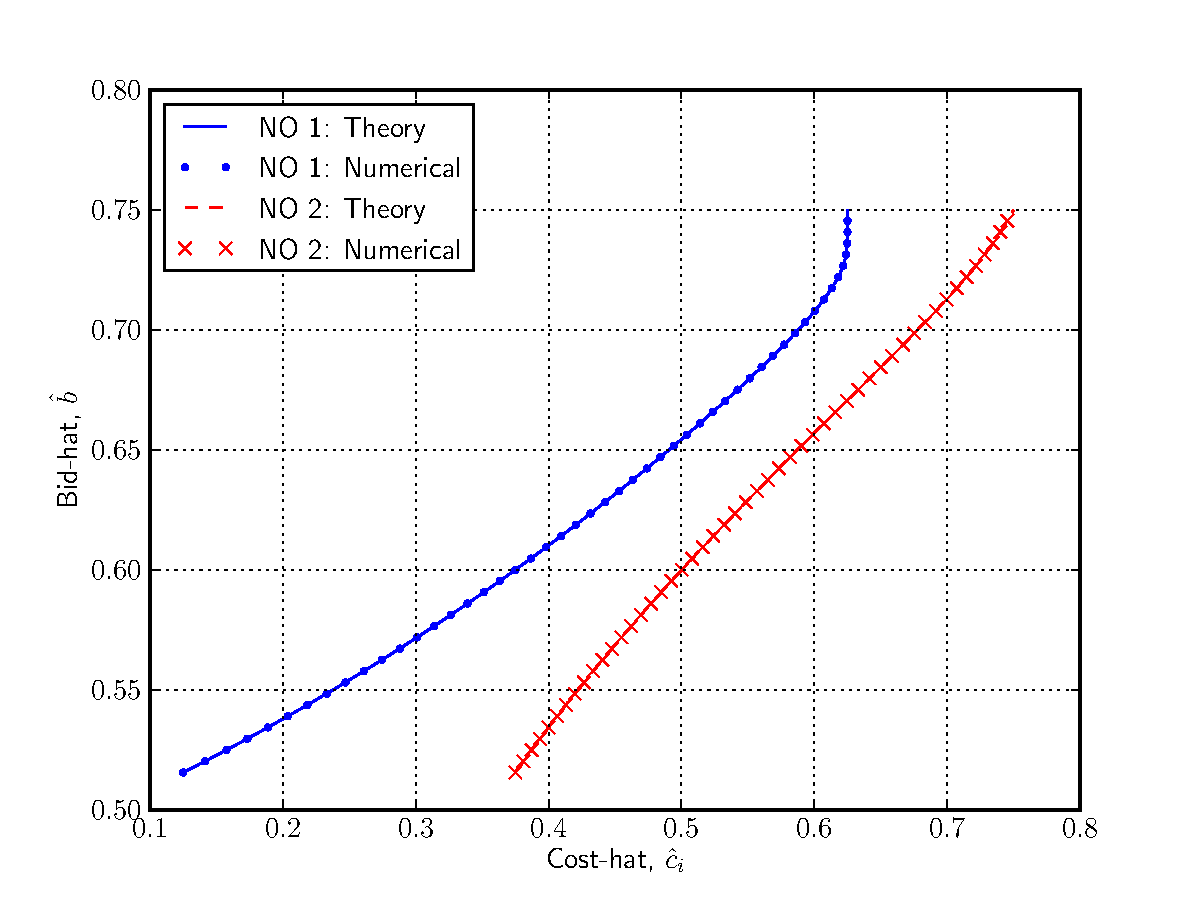
\includegraphics[width=\figsize]{Indirect/Figures/forward_shooting_verification}
  \caption{FSM solution to the bidding problem characterised by: $w=0.5$, $r_1 = 0.25$, and $r_2 = 0.75$ agreeing with the closed-form solution}
  \label{fig:forward_shooting_verification_indirect}
  \vspace{10mm}
  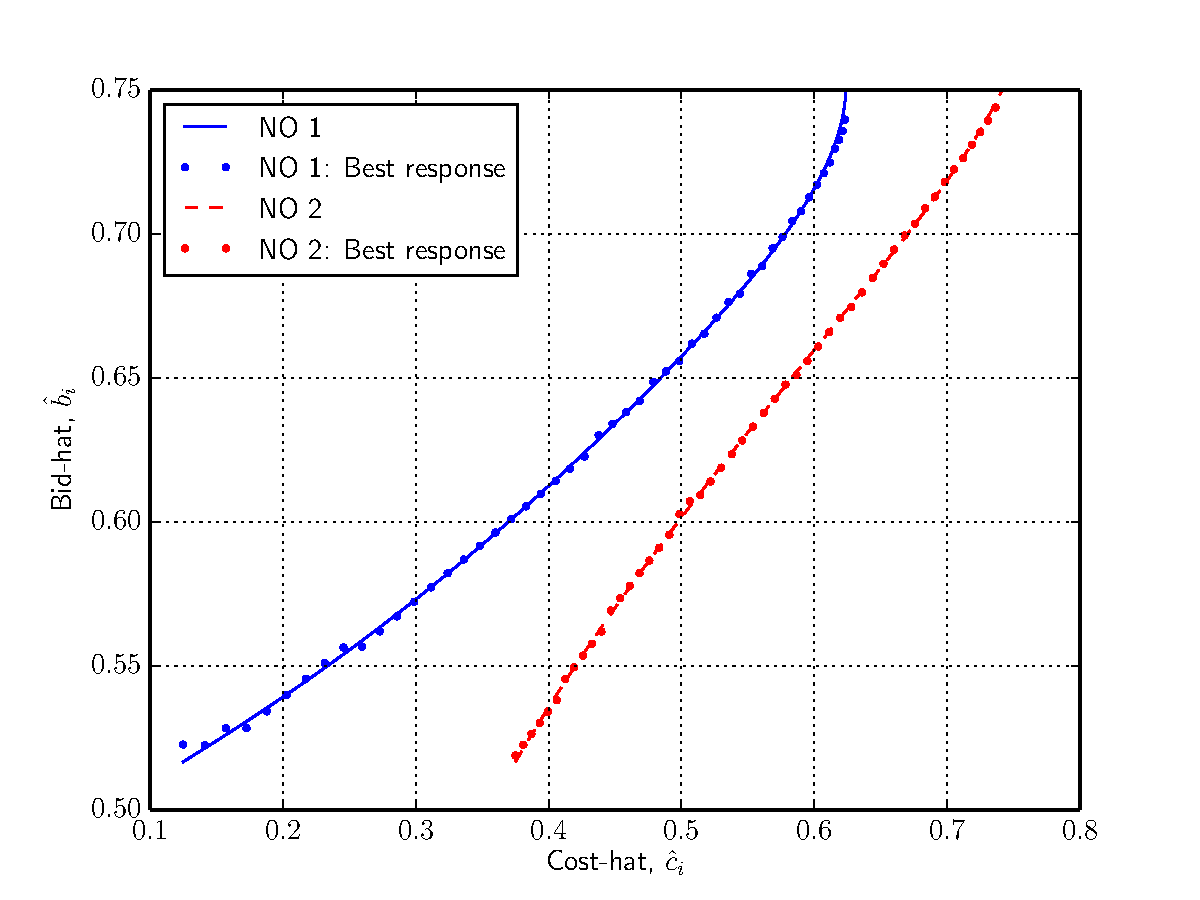
\includegraphics[width=\figsize]{Indirect/Figures/polynomial_projection_verification}
  \caption{PPM solution to the bidding problem characterised by: $w=0.5$, $r_1 = 0.25$, and $r_2 = 0.75$ agreeing with the closed-form solution}
  \label{fig:polynomial_projection_verification_indirect}
\end{figure}

Note, however, that this does not prove that the algorithms will provide correct results for any number of network operators. On the contrary, it merely suggests that the implementation of the algorithms passed basic sanity check. Therefore, in what follows, for each produced output, it will be verified whether the numerically approximated bidding strategies satisfy the sufficiency condition for an equilibrium; that is, whether the numerically derived bidding strategy for each network operator is a best response to the bidding strategies of the remaining network operators. If the derived bidding strategies constitute best responses that are mutually consistent, then they constitute an approximate Bayesian Nash equilibrium.

In the first examined scenario, there are 3 network operators characterised by reputation ratings as summarised in Table~\ref{tab:approximation_scenario_3_indirect}. Furthermore, the price weight is set to $0.75$. \annotate{C5.1}{Figures~\ref{fig:forward_shooting_3_sufficiency_indirect}~and~\ref{fig:polynomial_projection_3_sufficiency_indirect} depict the results of the approximation generated by the FSM and the PPM methods respectively.} Both approximation methods yield virtually the same estimate of the lower bound on bids, $\underline{\hat{b}}\approx 0.375$. In the FSM case, the approximation diverges in the very near proximity of $\bar{\hat{b}}$, and therefore, the approximation satisfies the sufficiency only until $b$ reaches a close neighbourhood of $\bar{\hat{b}}$. This is due to the fact that the system of ODEs does not satisfy Lipschitz condition as $b$ approaches $\bar{\hat{b}}$. The PPM method, on the other hand, eliminates this problem entirely, and the approximation satisfies sufficiency for all $b\in[\underline{\hat{b}},\bar{\hat{b}}]$.

\begin{table}[t]
  \caption{Bidding scenario with 3 network operators}
  \vspace{0.5cm}
  \begin{tabular*}{0.5\columnwidth}[L]{@{\extracolsep{\fill}}r c c}
    \hlx{vhv}
    & \textbf{Price weight}, $w$ & \textbf{Reputation rating}, $r_i$\\
    \hlx{vhv}
    \textbf{Network operator 1} & \multirow{3}{*}{$0.75$} & $0.25$\\
    \textbf{Network operator 2} & & $0.5$\\
    \textbf{Network operator 3} & & $0.75$\\
    \hlx{vhs}
  \end{tabular*}
  \label{tab:approximation_scenario_3_indirect}
\end{table}

\begin{figure}[p!]
  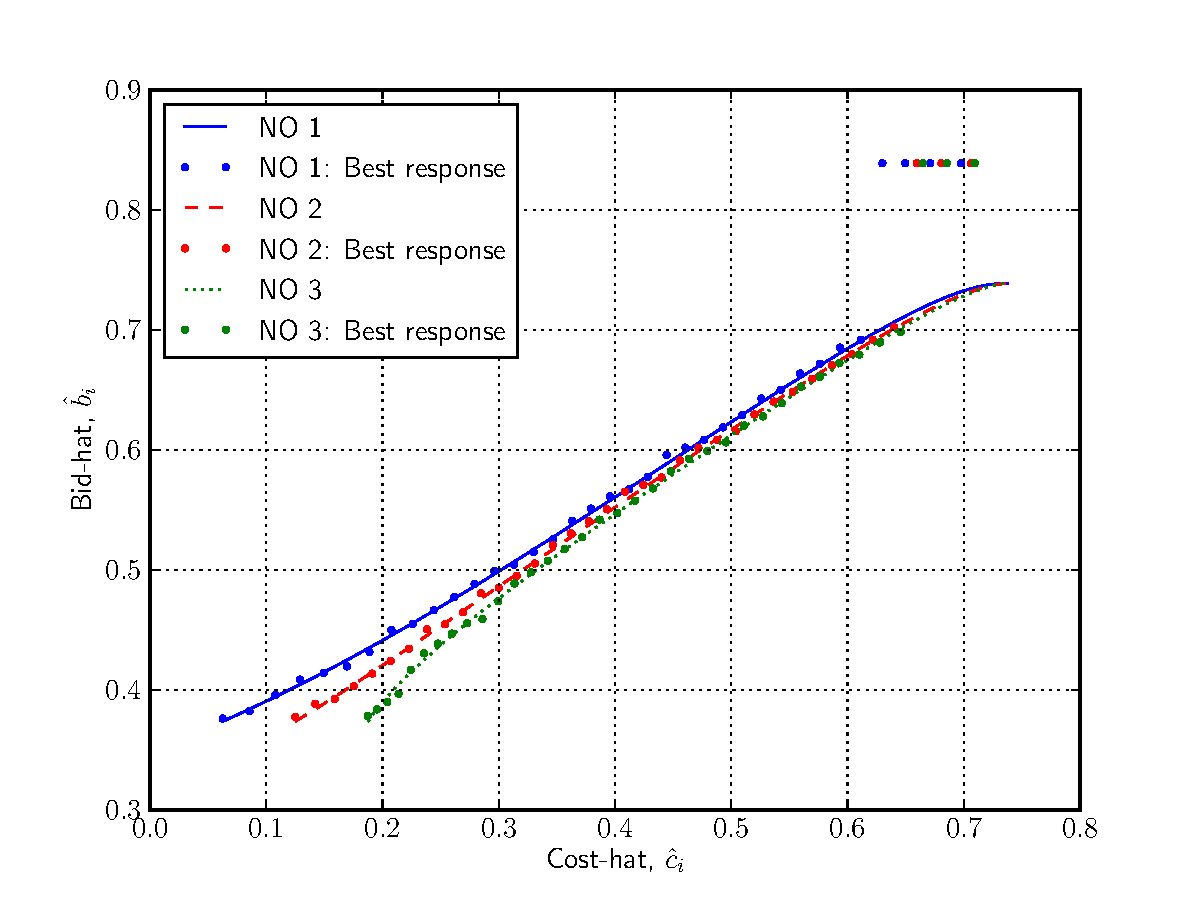
\includegraphics[width=\figsize]{Indirect/Figures/forward_shooting_3_sufficiency}
  \caption{FSM solution to the bidding problem characterised by: $w=0.75$, $r_1 = 0.25$, $r_2 = 0.5$, and $r_3 = 0.75$. The solution satisfies the sufficiency condition for all~$\hat{b}$ except~$\hat{b}$'s in the close neighbourhood of~$\bar{\hat{b}}$.}
  \label{fig:forward_shooting_3_sufficiency_indirect}
  \vspace{10mm}
  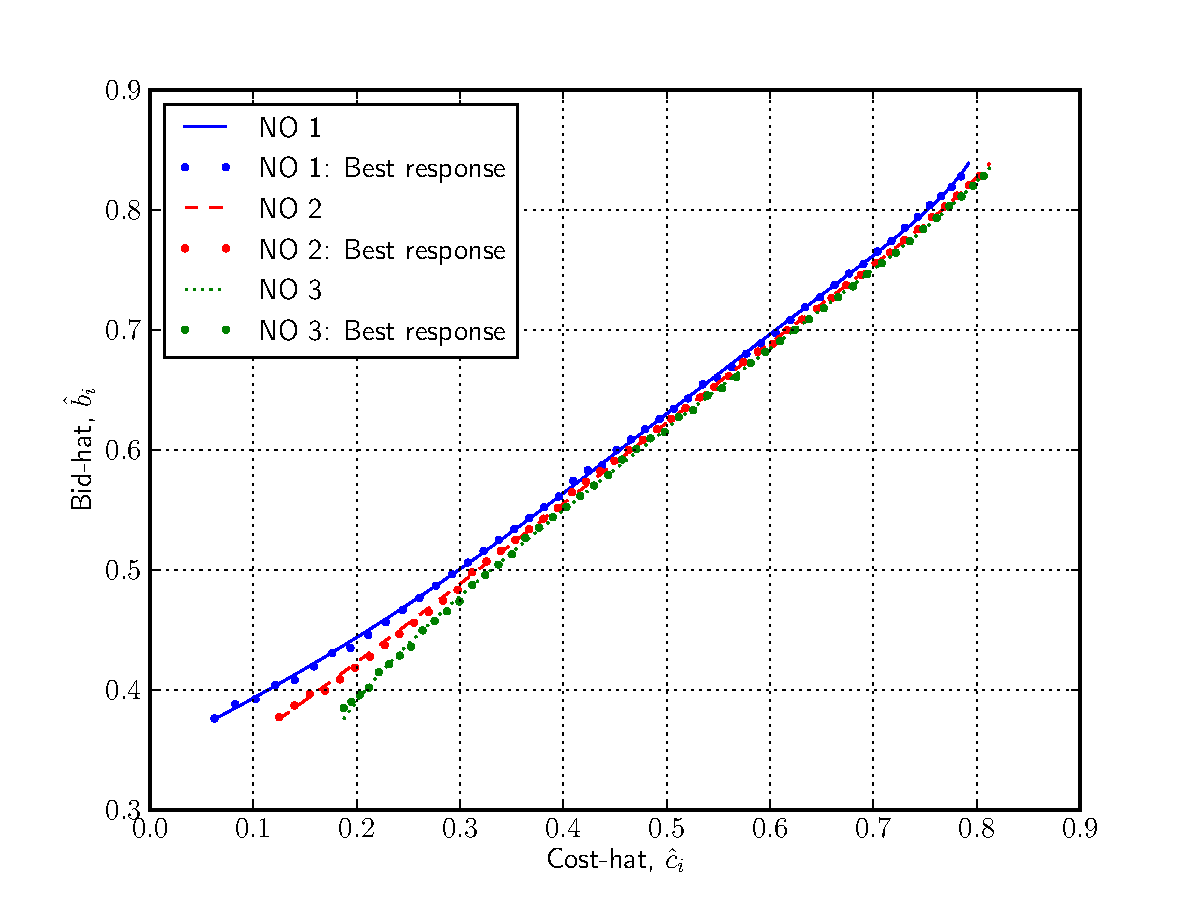
\includegraphics[width=\figsize]{Indirect/Figures/polynomial_projection_3_sufficiency}
  \caption{PPM solution to the bidding problem characterised by: $w=0.75$, $r_1 = 0.25$, $r_2 = 0.5$, and $r_3 = 0.75$. The solution satisfies the sufficiency condition for all~$\hat{b}$.}
  \label{fig:polynomial_projection_3_sufficiency_indirect}
\end{figure}

In the second examined scenario, there are 4 network operators characterized by reputation ratings as summarized in Table~\ref{tab:approximation_scenario_4_indirect}. Furthermore, the price weight is set to $0.85$. \annotate{C5.1}{Figures~\ref{fig:forward_shooting_4_sufficiency_indirect}~and~\ref{fig:polynomial_projection_4_sufficiency_indirect} depict the results of the approximation generated by the FSM and PPM methods respectively.} Both approximation methods yield virtually the same estimate of the lower bounds on bids, $\underline{\hat{b}}\approx 0.38$. Similarly to the bidding scenario with 3 network operators, in the FSM method case, the approximation diverges in the very near proximity of $\bar{\hat{b}}$, and therefore, the approximation satisfies the sufficiency only until $b$ reaches a close neighbourhood of $\bar{\hat{b}}$. In the PPM method case, the approximation satisfies sufficiency for all $b\in[\underline{\hat{b}},\bar{\hat{b}}]$.

\begin{table}[t]
  \caption{Bidding scenario with 4 network operators}
  \vspace{0.5cm}
  \begin{tabular*}{0.5\columnwidth}[L]{@{\extracolsep{\fill}}r c c}
    \hlx{vhv}
    & \textbf{Price weight}, $w$ & \textbf{Reputation rating}, $r_i$\\
    \hlx{vhv}
    \textbf{Network operator 1} & \multirow{4}{*}{$0.85$} & $0.2$\\
    \textbf{Network operator 2} & & $0.4$\\
    \textbf{Network operator 3} & & $0.6$\\
    \textbf{Network operator 4} & & $0.8$\\
    \hlx{vhs}
  \end{tabular*}
  \label{tab:approximation_scenario_4_indirect}
\end{table}

\begin{figure}[p!]
  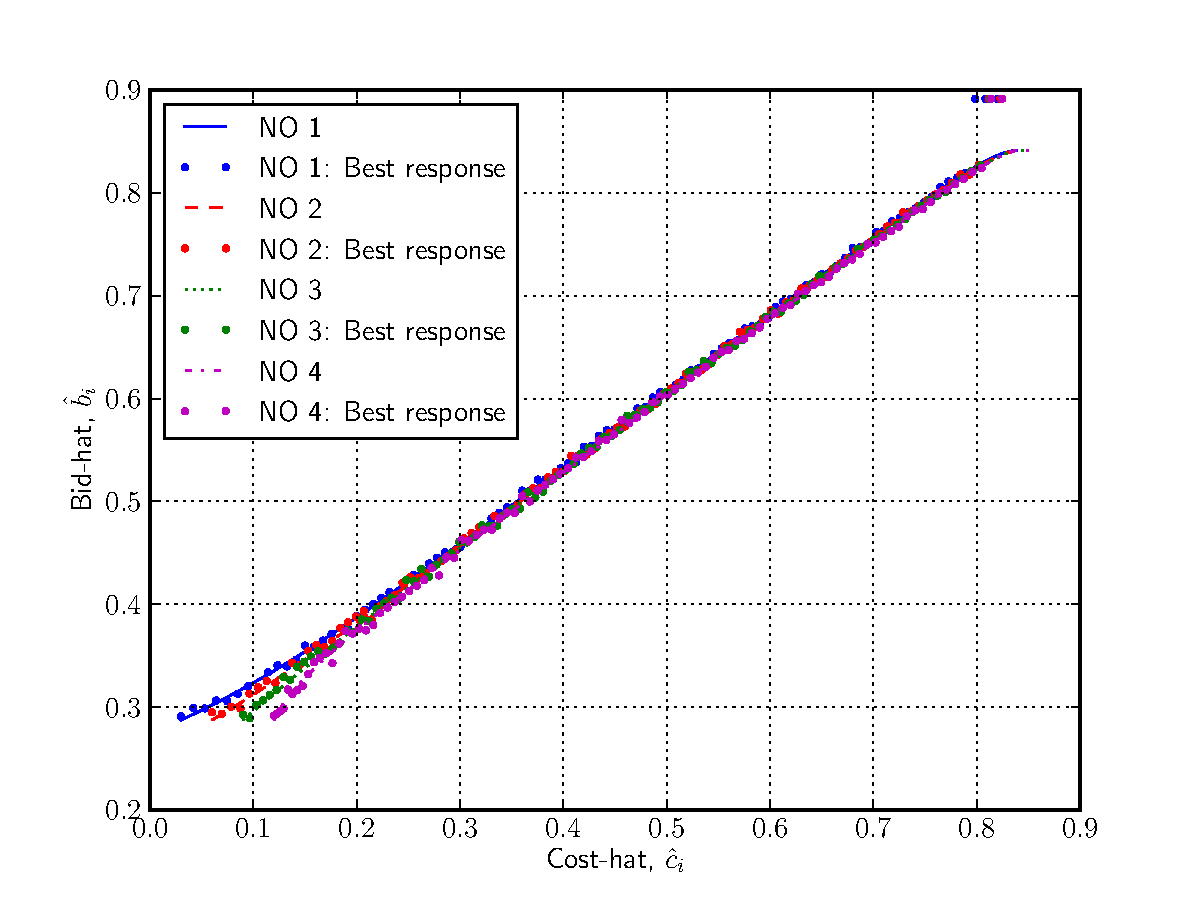
\includegraphics[width=\figsize]{Indirect/Figures/forward_shooting_4_sufficiency}
  \caption{FSM solution to the bidding problem characterised by: $w=0.85$, $r_1 = 0.2$, $r_2 = 0.4$, $r_3 = 0.6$, and $r_4=0.8$. The solution satisfies the sufficiency condition for all~$\hat{b}$ except~$\hat{b}$'s in the close neighbourhood of~$\bar{\hat{b}}$.}
  \label{fig:forward_shooting_4_sufficiency_indirect}
  \vspace{10mm}
  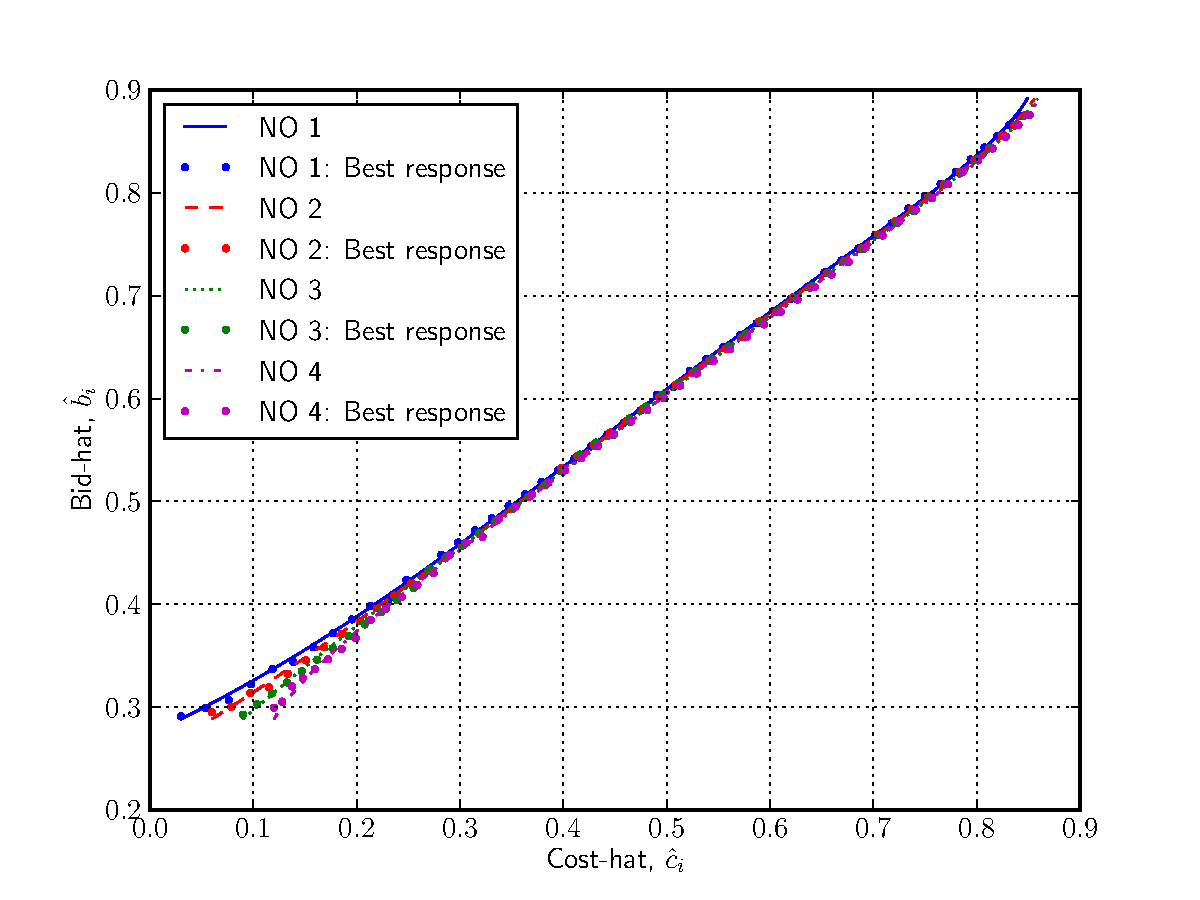
\includegraphics[width=\figsize]{Indirect/Figures/polynomial_projection_4_sufficiency}
  \caption{PPM solution to the bidding problem characterised by: $w=0.85$, $r_1 = 0.2$, $r_2 = 0.4$, $r_3 = 0.6$, and $r_4=0.8$. The solution satisfies the sufficiency condition for all~$\hat{b}$.}
  \label{fig:polynomial_projection_4_sufficiency_indirect}
\end{figure}
% subsection approximation_results (end)

In this section, the FSM and PPM numerical algorithms were described, and two exemplary bidding scenarios were analysed for which the equilibrium bidding strategies were generated using the aforementioned algorithms. It should be noted, however, that one of the key assumptions of this section was $\underline{\hat{c}}_i\leq \hat{c}(\underline{\hat{b}})$ for all network operators $i\in N$, which restricted the choice of the price weight and the reputation ratings to a set satisfying $w\geq 1 - \sfrac{1}{(10r_n - 9r_2 - r_1 + 1)}$. In the following section, this assumption is relaxed by allowing cases such that $\hat{c}(\underline{\hat{b}}) < \underline{\hat{c}}_i < \bar{\hat{b}}$ for at least one network operator $i\in N$. In other words, all nontrivial equilibria characterised by Proposition~\ref{prop:characterization_of_the_equilibrium_indirect} are considered. Furthermore, a numerical algorithm which is able to generate equilibrium bidding strategies under the relaxed assumption is presented.
% section numerical_analysis_indirect (end)

\section{Extended Numerical Analysis} % (fold)
\label{sec:extended_numerical_analysis_indirect}
Suppose $\hat{c}(\underline{\hat{b}}) < \underline{\hat{c}}_i < \bar{\hat{b}}$ for at least one $i\in N$, and let all the remaining assumptions of Section~\ref{sec:numerical_analysis_indirect} hold. To be more specific, let $w\in (0.5,1.0)$ for all $r_i\in[0,1], i\in N$ such that $r_1\leq\cdots\leq r_n$ with at least one inequality strict.

In what follows, a numerical algorithm which improves upon the algorithms considered in Section~\ref{sec:numerical_analysis_indirect} is presented: the extended forward shooting method (EFSM). Furthermore, the numerically approximated equilibrium bidding strategies for two bidding scenarios generated using the algorithm are analysed. \annotate{C5.19}{It is, furthermore, assumed without loss of generality that network operator 1 is characterised by the lowest reputation rating, network operator 2 by the second lowest, and so on. Hence, $\underline{\hat{c}}_1\leq \underline{\hat{c}}_2\leq \underline{\hat{c}}_i$ and $\bar{\hat{c}}_1\leq \bar{\hat{c}}_2\leq \bar{\hat{c}}_i$ for all $i\geq 2$.}

\subsection{Extended Forward Shooting Method} % (fold)
\label{sub:extended_forward_shooting_method_indirect}
The EFSM method extends the FSM method by effectively implementing the reasoning behind the bidding extension characterised by Lebrun~\cite{Lebrun2006} (see Section~\ref{sec:numerical_analysis_indirect} for a description of the extension). \annotate{C5.23}{To the best of the author's knowledge, the EFSM method developed in this thesis is the only numerical algorithm that considers all nontrivial equilibria to the system of ODEs in Equation~\eqref{eq:foc_ode_indirect} with lower and upper boundary conditions in Equations~\eqref{eq:foc_ode_lower_boundary_indirect}~and~\eqref{eq:foc_ode_upper_boundary_indirect} respectively.}

Similarly to the FSM method, the EFSM aims at finding the best approximation of the lower bound on bids, $\underline{\hat{b}}'$ say, by successively picking a value from the feasible interval $(\underline{\hat{c}}_2,\bar{\hat{b}})$, and verifying whether a numerical solution to the initial value problem
\begin{equation}
  \label{eq:efsm_initial_value_problem_indirect}
  \begin{array}{ll}
    \displaystyle\frac{d}{db}\hat{c}_i(b) &= \displaystyle\frac{1 - F_i(\hat{c}_i(b))}{f_i(\hat{c}_i(b))}\left[ \frac{1}{n-1}\sum_{k=1}^n\frac{1}{b - \hat{c}_k(b)} - \frac{1}{b - \hat{c}_i(b)} \right] \\[2ex]
    \hat{c}_i(\underline{\hat{b}}') &= \min\{\underline{\hat{c}}_i, \hat{c}(\underline{\hat{b}}')\}
  \end{array}
\end{equation}
\annotate{C5.14}{for all $i\in N$ satisfies the following three conditions: 1) it is a function mapping $[\underline{\hat{b}}',\bar{\hat{b}}]$ into $[\min\{\underline{\hat{c}}_i, \hat{c}(\underline{\hat{b}}')\}, \bar{\hat{c}}_i]$, that is,
\begin{equation}
  \label{eq:efsm_condition_1_indirect}
  s_i: [\underline{\hat{b}}', \bar{\hat{b}}]\to [\min\{\underline{\hat{c}}_i, \hat{c}(\underline{\hat{b}}')\}, \bar{\hat{c}}_i];
\end{equation}
2) it is monotonically increasing everywhere except possibly at $\bar{\hat{b}}$, that is,
\begin{equation}
  \label{eq:efsm_condition_2_indirect}
  b_1 < b_2\implies s_i(b_1) < s_i(b_2) \textrm{ for all }b_1,b_2\in [\underline{\hat{b}}', \bar{\hat{b}});
\end{equation}
and 3) each function value is strictly lower than its argument except possibly at $\bar{\hat{b}}$, that is,
\begin{equation}
  \label{eq:efsm_condition_3_indirect}
  s_i(b) < b \textrm{ for all }b\in [\underline{\hat{b}}', \bar{\hat{b}}).
\end{equation}}

\begin{algorithm}[p]
\caption{Extended forward shooting method}
\label{alg:extended_forward_shooting_method_indirect}
\begin{algorithmic}[1]
\Require{$\epsilon\in (0, \bar{\hat{b}} - \underline{\hat{c}}_2)$; $low, high\in [\underline{\hat{c}}_2, \bar{\hat{b}}]$ such that $low\leq high$}
\Ensure{Approximation to $\underline{\hat{b}}$}
  \Statex
  \Let{$low$}{$\underline{\hat{c}}_2$}
  \Let{$high$}{$\bar{\hat{b}}$}
  \Statex
  \While{$high-low > \epsilon$}
    \Let{$guess$}{$0.5\cdot(low + high)$}
    \Let{$(k,\hat{c})$}{\Call{estimateKC}{$guess,\underline{\hat{c}}_1,\ldots,\underline{\hat{c}}_n$}}
    \Let{$bids$}{$[guess, \bar{\hat{b}})$}
    \Let{$(costs_1,\dotsc,costs_n)$}{solve~\eqref{eq:efsm_initial_value_problem_indirect} with initial value $\underline{\hat{b}}' = guess$}
    \StatexIndent[7.5]{evaluated at points $b\in bids$, and $k(\underline{\hat{b}}) = k$}
    \StatexIndent[7.5]{and $\hat{c}(\underline{\hat{b}}) = \hat{c}$}
    \If{$(bids,costs_i)$ satisfies~\eqref{eq:efsm_condition_1_indirect}, \eqref{eq:efsm_condition_2_indirect} and \eqref{eq:efsm_condition_3_indirect} for all $i\gets 1$ to $n$}
      \Let{$high$}{$guess$}
    \Else
      \Let{$low$}{$guess$}
    \EndIf
  \EndWhile
  \Statex
  \Let{$\underline{\hat{b}}'$}{$0.5\cdot(low + high)$}
\end{algorithmic}
\end{algorithm}

\begin{algorithm}[p]
\caption{Function for estimating $k(\underline{\hat{b}})$ and $\hat{c}(\underline{\hat{b}})$}
\label{alg:function_estimate_k_c_indirect}
\begin{algorithmic}[1]
\Require{Estimate of $\underline{\hat{b}}$; $\underline{\hat{c}}_i$ for all $i\in N$}
\Ensure{$k(\underline{\hat{b}})\in \{2,\ldots,n\}$; $\hat{c}(\underline{\hat{b}})$ computed according to~\eqref{eq:lower_bound_bids_cost_indirect}}
  \Statex
  \Function{estimateKC}{$\underline{\hat{b}},\underline{\hat{c}}_1,\ldots,\underline{\hat{c}}_n$}
    \For{$k = 2 \to n$}
      \Let{$\hat{c}(\underline{\hat{b}})$}{compute using~\eqref{eq:lower_bound_bids_cost_indirect} with $k(\underline{\hat{b}}) = k$}
      \If{$k<n$}
        \If{$\underline{\hat{c}}_k\leq \hat{c}(\underline{\hat{b}})\land\hat{c}(\underline{\hat{b}})<\underline{\hat{c}}_{k+1}$}
          \State{\textbf{break}}
        \EndIf
      \EndIf
    \EndFor
    \State\Return{$(k,\hat{c}(\underline{\hat{b}}))$}
  \EndFunction
\end{algorithmic}
\end{algorithm}

The pseudo-code for the EFSM is shown in listing Algorithm~\ref{alg:extended_forward_shooting_method_indirect}. The flow of the algorithm is almost exactly the same as for the FSM. The main differences are twofold: the algorithm estimates $k(\underline{\hat{b}}')$ and $\hat{c}(\underline{\hat{b}}')$ (line 6); \annotate{C5.3}{and the algorithm solves the system~\eqref{eq:efsm_initial_value_problem_indirect} using the reasoning behind the bidding extension characterised by Lebrun~\cite{Lebrun2006} and described below (line 8).}

Listing Algorithm~\ref{alg:function_estimate_k_c_indirect} depicts the pseudo-code for the function `estimateKC' which estimates $k(\underline{\hat{b}}')$ and $\hat{c}(\underline{\hat{b}}')$. It takes as an input an estimate of the lower bound on bids, $\underline{\hat{b}}'$, and the set of lower extremities $\{\underline{\hat{c}}_i\}$ for all $i\in N$. The function then iterates over $k\in\{2,\ldots,n\}$, and for each $k$ it computes $\hat{c}(\underline{\hat{b}}')$ according to Equation~\eqref{eq:lower_bound_bids_cost_indirect}. If $k<n$ and $\hat{c}(\underline{\hat{b}}')$ satisfies~\eqref{eq:bounds_lower_bound_bids_cost_indirect}, then the function returns that particular pair of values $(k, \hat{c}(\underline{\hat{b}}'))$ such that $2\leq k < n$. Otherwise, $k=n$ is returned which reduces system~\eqref{eq:efsm_initial_value_problem_indirect} to~\eqref{eq:fsm_initial_value_problem_indirect}, and EFSM to FSM.

\begin{figure}[t]
  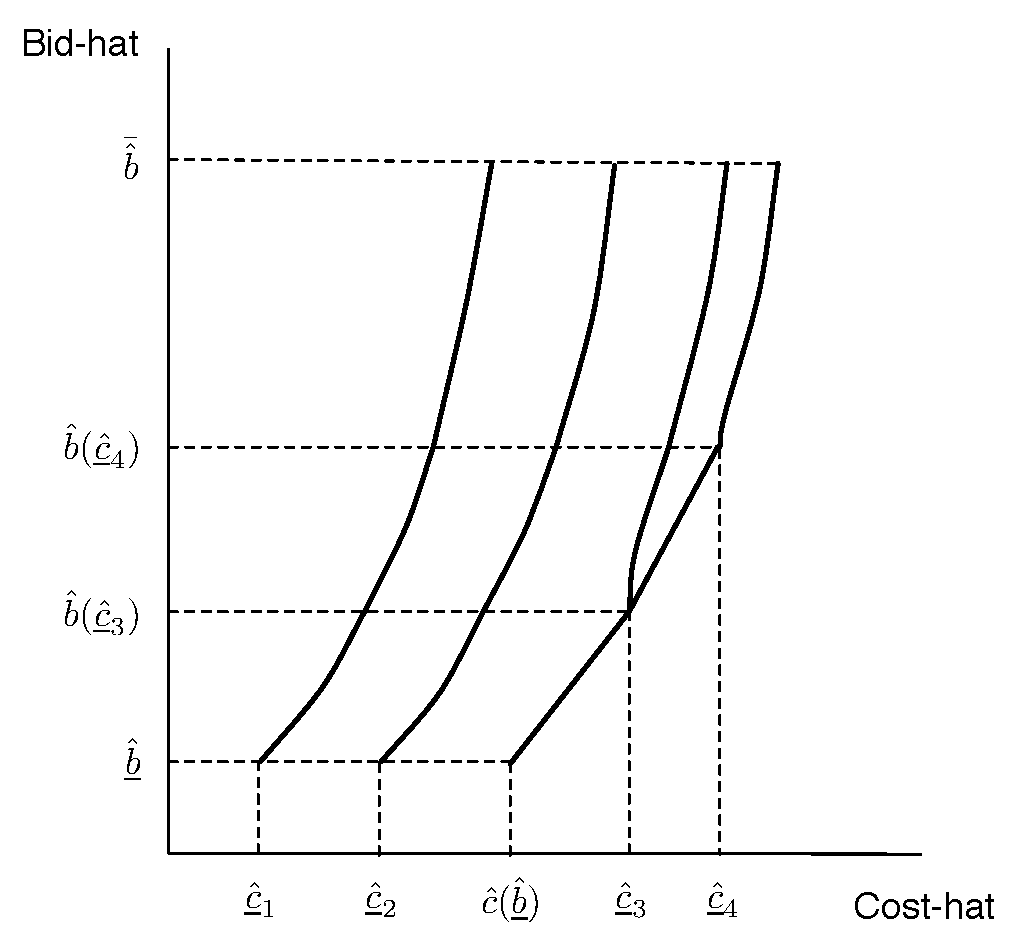
\includegraphics[width=\figsize]{Indirect/Figures/lebrun_solution}
  \caption{The reasoning behind the bidding extension characterised by Lebrun~\cite{Lebrun2006} captured by the EFSM method}
  \label{fig:lebrun_solution_indirect}
\end{figure}

\annotate{C5.3}{In order to describe how the algorithm solves the system~\eqref{eq:efsm_initial_value_problem_indirect}, suppose there are $n=4$ network operators.} The following argument can easily be adapted to the case of $n=3$ or $n>4$ network operators. Furthermore, suppose that
\begin{equation}
  \underline{\hat{c}}_1 < \underline{\hat{c}}_2 < \hat{c}(\underline{\hat{b}}) < \underline{\hat{c}}_3 < \underline{\hat{c}}_4.
\end{equation}
The method comprises three stages as depicted in Figure~\ref{fig:lebrun_solution_indirect}.

\begin{description}
\item[Stage 1] Since $\underline{\hat{c}}_1 < \underline{\hat{c}}_2 < \hat{c}(\underline{\hat{b}}) < \underline{\hat{c}}_3 < \underline{\hat{c}}_4$, then $k(\underline{\hat{b}}) = 2$, and hence, network operators 1 and 2 solve
\begin{equation}
  \label{eq:efsm_lebrun_ode_1_indirect}
  \begin{array}{ll}
    \displaystyle\frac{d}{db}\hat{c}_i(b) &= \displaystyle\frac{1 - F_i(\hat{c}_i(b))}{f_i(\hat{c}_i(b))}\left[ \frac{1}{k(\underline{\hat{b}})-1}\sum_{k=1}^{k(\underline{\hat{b}})}\frac{1}{b - \hat{c}_k(b)} - \frac{1}{b - \hat{c}_i(b)} \right] \\[2ex]
    \hat{c}_i(\underline{\hat{b}}) &= \underline{\hat{c}}_i
  \end{array},
\end{equation}
while network operators 3 and 4 solve
\begin{equation}
  \label{eq:efsm_lebrun_ext_1_indirect}
  \hat{c}_i(b) = b - \frac{k(\underline{\hat{b}}) - 1}{\sum_{j=1}^{k(\underline{\hat{b}})} \frac{1}{b-\hat{c}_j(b)}}.
\end{equation}
The system~\eqref{eq:efsm_lebrun_ode_1_indirect} is solved for all $b\in[\underline{\hat{b}},\bar{\hat{b}}]$, and the approximation is then used to solve~\eqref{eq:efsm_lebrun_ext_1_indirect}. However, only bid values such that $\underline{\hat{b}} \leq b\leq \hat{b}_3(\underline{\hat{c}}_3)$ are kept, where $\hat{c}_3(\hat{b}_3(\underline{\hat{c}}_3)) = \underline{\hat{c}}_3$ maps into network operator's 3 cost-hat.

Note that the solution to~\eqref{eq:efsm_lebrun_ext_1_indirect} depends only on $k(\underline{\hat{b}})$ and the solution to~\eqref{eq:efsm_lebrun_ode_1_indirect}. Therefore, both network operator 3 and 4 are characterised by the same set of values (Stage 1, Figure~\ref{fig:lebrun_solution_indirect}).

\item[Stage 2] Next, $k(\underline{\hat{b}})$ is incremented by $1$ over the previous value, and the procedure in Stage 1 is repeated with this difference that now network operators 1, 2 and 3 solve system~\eqref{eq:efsm_lebrun_ode_1_indirect} while network operator 4 solves~\eqref{eq:efsm_lebrun_ext_1_indirect}. The system~\eqref{eq:efsm_lebrun_ode_1_indirect} is solved for $b\in [\hat{b}_3(\underline{\hat{c}}_3), \bar{\hat{b}}]$, but only bid values such that $\hat{b}_3(\underline{\hat{c}}_3)\leq b\leq \hat{b}_4(\underline{\hat{b}}_4)$ are kept (Stage 2, Figure~\ref{fig:lebrun_solution_indirect}).

\item[Stage 3] Finally, all network operators solve the system~\eqref{eq:efsm_lebrun_ode_1_indirect} for bid values $b\in [\hat{b}_4(\underline{\hat{c}}_4),\bar{\hat{b}}]$ (Stage 3, Figure~\ref{fig:lebrun_solution_indirect}).
\end{description}

In each stage, the system of ODEs in Equation~\eqref{eq:efsm_lebrun_ode_1_indirect} can be solved numerically using any type of finite-difference methods, such as Euler or Runge-Kutta methods. The results presented in this section were obtained using the GSL implementation of the Embedded-Runge-Kutta-Fehlberg (4, 5) method~\cite{GSL}.

Furthermore, similarly to the implementation of the FSM and PPM methods, in the implementation of EFSM, it was assumed that
\begin{equation}
  F_i(x) = \frac{x - \underline{\hat{c}}_i}{\bar{\hat{c}}_i - \underline{\hat{c}}_i} \quad\textrm{and}\quad f_i(x) = \frac{1}{\bar{\hat{c}}_i - \underline{\hat{c}}_i}
\end{equation}
for all $i\in N$ and $x\in\mathbb{R}$. The discussion of the consequences arising from this simplifying assumption can be found in Section~\ref{sub:forward_shooting_method_indirect}.

% subsection extended_forward_shooting_method_indirect (end)

\subsection{Approximation Results} % (fold)
\label{sub:extended_approximation_results_indirect}
This subsection presents the approximation results for two bidding scenarios with 3 and 4 network operators. \annotate{C5.16}{Similarly to the algorithms presented in Section~\ref{sec:numerical_analysis_indirect}, the EFSM method was tested for correct implementation using the same procedure as presented in Section~\ref{sec:numerical_analysis_indirect}. However, since the verification results match exactly those presented in Figure~\ref{fig:forward_shooting_verification_indirect}, their discussion is omitted from this section.}

In the first examined scenario, there are 3 network operators characterised by reputation ratings summarised in Table~\ref{tab:approximation_scenario_ext_3_indirect}. Furthermore, the price weight is set to $0.55$. \annotate{C5.1}{Figure~\ref{fig:efs_3_sufficiency_indirect} depicts the results of the approximation generated by the EFSM method.} The method yields an estimate of the lower bound on bids of $\underline{\hat{b}}\approx 0.407$, and satisfies the sufficiency for all $b\in[\underline{\hat{b}},\bar{\hat{b}}]$. It is worth noting that, as expected, the bidding scenario comprises two stages (cf.~Figure~\ref{fig:lebrun_solution_indirect}): stage 1 such that $\hat{b}\in [0.407, 0.43]$ where network operators 1 and 2 are competing against each other only, and network operator 3 is characterised by the bidding extension given by Equation~\eqref{eq:efsm_lebrun_ext_1_indirect}; and stage 2 such that $\hat{b}\in [0.43, 0.71]$ where all network operators are competing against each other, and are solving the system in Equation~\eqref{eq:efsm_lebrun_ode_1_indirect}.

\begin{table}[t]
  \caption{Bidding scenario with 3 network operators}
  \vspace{0.5cm}
  \begin{tabular*}{0.5\columnwidth}[L]{@{\extracolsep{\fill}}r c c}
    \hlx{vhv}
    & \textbf{Price weight}, $w$ & \textbf{Reputation rating}, $r_i$\\
    \hlx{vhv}
    \textbf{Network operator 1} & \multirow{3}{*}{$0.55$} & $0.25$\\
    \textbf{Network operator 2} & & $0.5$\\
    \textbf{Network operator 3} & & $0.75$\\
    \hlx{vhs}
  \end{tabular*}
  \label{tab:approximation_scenario_ext_3_indirect}
\end{table}

\begin{figure}[t]
  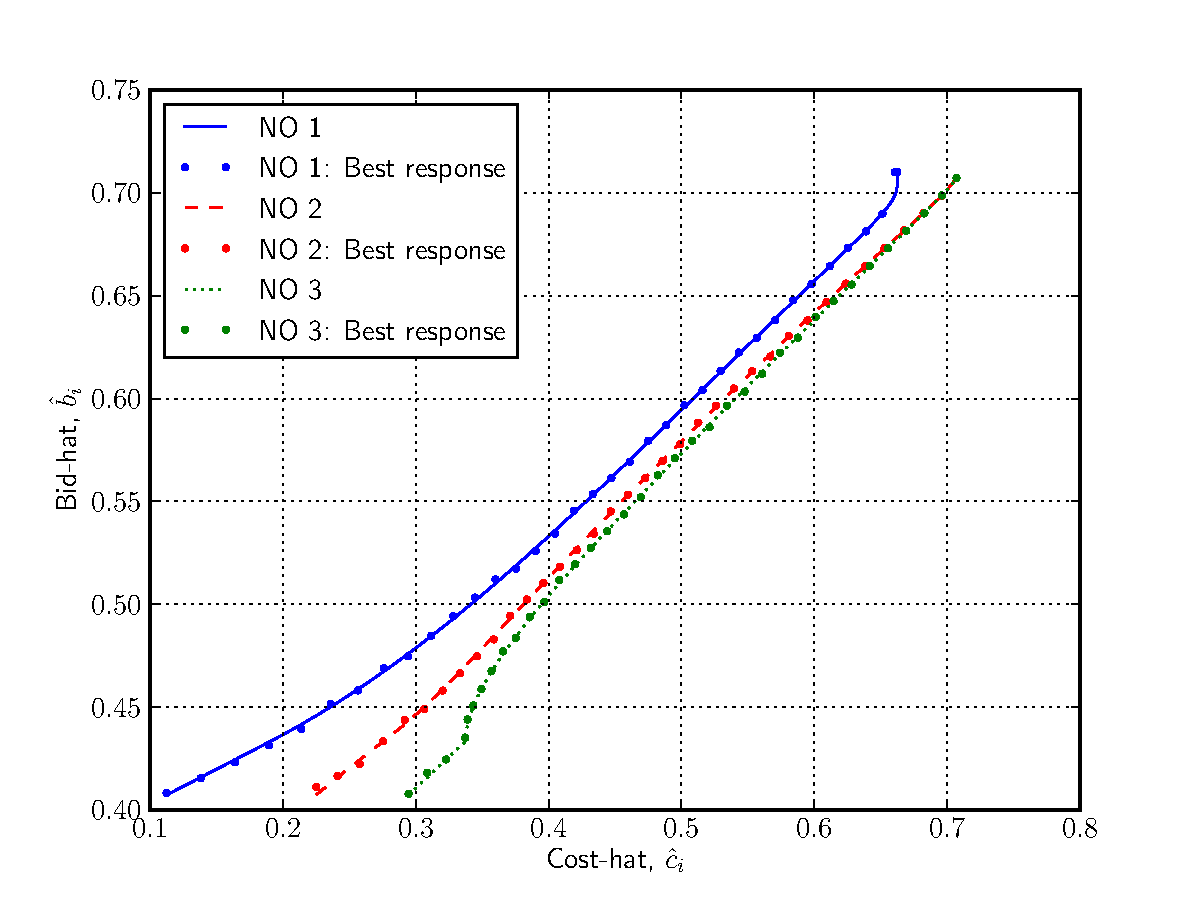
\includegraphics[width=\figsize]{Indirect/Figures/efs_3_sufficiency}
  \caption{EFSM solution to the bidding problem characterised by: $w=0.55$, $r_1 = 0.25$, $r_2 = 0.5$, and $r_3 = 0.75$. The solution satisfies the sufficiency for all $\hat{b}$.}
  \label{fig:efs_3_sufficiency_indirect}
\end{figure}

In the second examined scenario, there are 4 network operators characterised by reputation ratings summarised in Table~\ref{tab:approximation_scenario_ext_4_indirect}. Furthermore, the price weight is set to $0.55$. \annotate{C5.1}{Figure~\ref{fig:efs_4_sufficiency_indirect} depicts the results for the approximation generated by EFSM.} The estimate of the lower bound on bids is $\underline{\hat{b}}\approx 0.353$, and the solution satisfies the sufficiency for all $b\in[\underline{\hat{b}},\bar{\hat{b}}]$. It is worth noting that, as expected, the bidding scenario comprises three stages (cf.~Figure~\ref{fig:lebrun_solution_indirect}): stage 1 such that $\hat{b}\in [0.353, 0.3625]$ where network operators 1 and 2 are competing against each other, while network operators 3 and 4 are characterised by the bidding extension given by Equation~\eqref{eq:efsm_lebrun_ext_1_indirect}; stage 2 such that $\hat{b}\in [0.3625, 0.43]$ where network operators 1, 2 and 3 are competing against each other, and network operator 4 is still characterised by the bidding extension, albeit different compared to the bidding extension established in stage 1; and stage 3 such that $\hat{b}\in [0.43, 0.675]$ where all network operators are competing against each other.

\begin{table}[t]
  \caption{Bidding scenario with 4 network operators}
  \vspace{0.5cm}
  \begin{tabular*}{0.5\columnwidth}[L]{@{\extracolsep{\fill}}r c c}
    \hlx{vhv}
    & \textbf{Price weight}, $w$ & \textbf{Reputation rating}, $r_i$\\
    \hlx{vhv}
    \textbf{Network operator 1} & \multirow{4}{*}{$0.55$} & $0.2$\\
    \textbf{Network operator 2} & & $0.4$\\
    \textbf{Network operator 3} & & $0.6$\\
    \textbf{Network operator 4} & & $0.8$\\
    \hlx{vhs}
  \end{tabular*}
  \label{tab:approximation_scenario_ext_4_indirect}
\end{table}

\begin{figure}[t]
  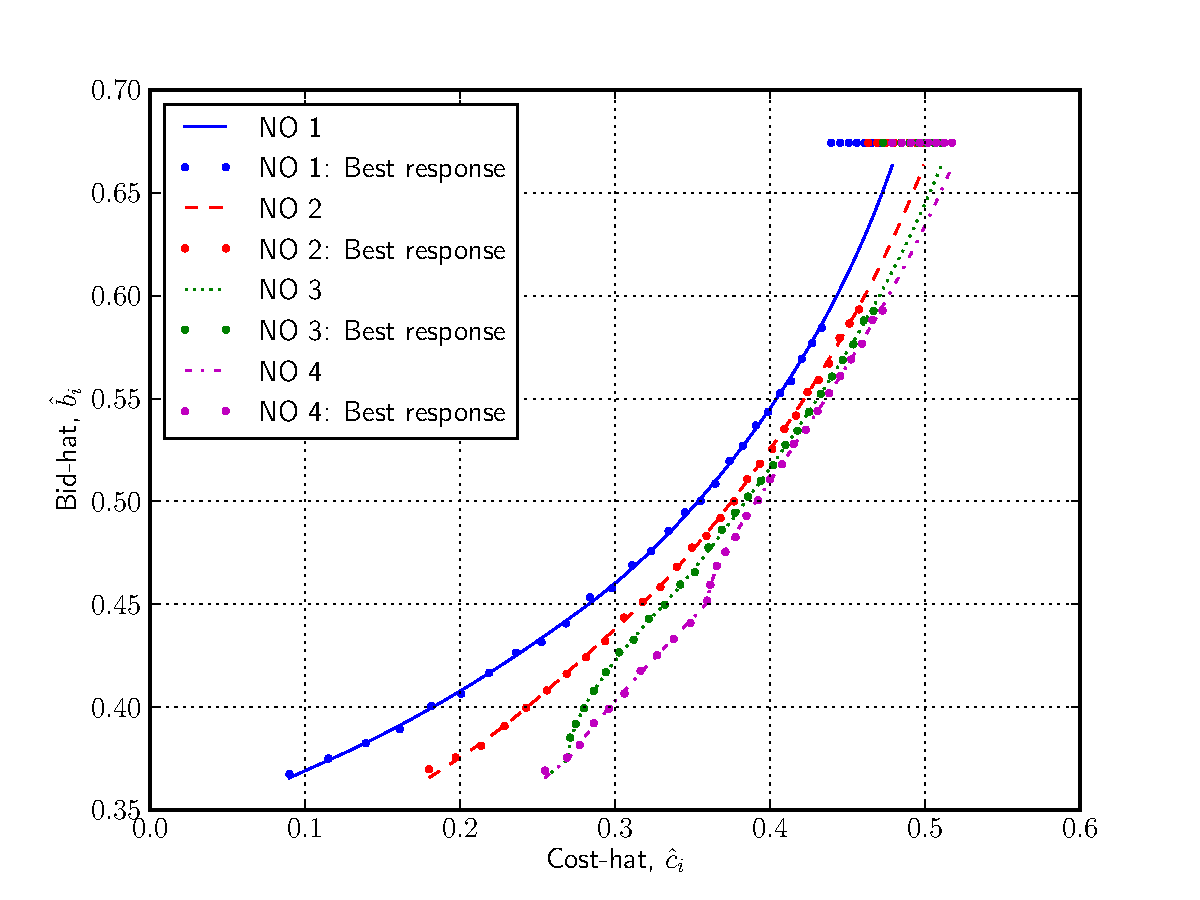
\includegraphics[width=\figsize]{Indirect/Figures/efs_4_sufficiency}
  \caption{EFSM solution to the bidding problem characterised by: $w=0.55$, $r_1 = 0.2$, $r_2 = 0.4$, $r_3 = 0.6$, and $r_4 = 0.8$. The solution satisfies the sufficiency for all $\hat{b}$.}
  \label{fig:efs_4_sufficiency_indirect}
\end{figure}
% subsection extended_approximation_results_indirect (end)

In this section, the EFSM numerical algorithm was outlined, and two exemplary bidding scenarios were analysed for which the equilibrium bidding strategies were generated by the aforementioned algorithms. The method ``completes'' the FSM and PPM methods in the sense that it permits for cases such that $\hat{c}(\underline{\hat{b}}) < \underline{\hat{c}}_i < \bar{\hat{b}}$ for at least one network operator $i\in N$, and hence, considers all nontrivial equilibria characterised by Proposition~\ref{prop:characterization_of_the_equilibrium_indirect}. It is an important improvement since otherwise only a very restricted subset of all possible bidding scenarios resulting in nontrivial equilibria could be considered and numerically approximated.
% section extended_numerical_analysis_indirect (end)

\section{Summary}
\label{sec:summary_indirect}
In this chapter, the bidding problem with symmetric cost distributions, as defined in Chapter~\ref{cha:direct}, was transformed into a bidding problem with asymmetric cost distributions. Following the transformation, the equilibrium bidding strategies for the generic case of $n$ network operators were formally characterised; that is, it was shown that the pure strategy Bayesian Nash equilibrium exists and is unique (Proposition~\ref{prop:characterization_of_the_equilibrium_indirect} and Corollary~\ref{cor:characterization_of_the_equilibrium_indirect}). \annotate{C5.24}{This is an important result as it proves that the DMP network selection mechanism is economically well-behaved since the equilibrium exists.}

\annotate{C5.24}{When restricted to $n=2$ network operators, the equilibrium bidding strategies were analytically derived. To aid in the derivation, it was necessary to assume that costs for the network operators were uniformly distributed. Given the lack of knowledge of the way the costs are distributed, it is standard practice to assume the probability of each cost to be uniform~\cite{Chung2004}. Nonetheless, such an assumption is limiting and it is highly likely it will not be representative of the reality. Furthermore, in the same case of $n=2$ network operators, the expected prices for the subscriber were analysed, and it was shown that, for any expected price, as the difference between the reputation ratings of the network operators increases, the price weight has to increase (or remain constant) in order to keep the expected price fixed. This observation carries very serious implications on the operation of the DMP, as the subscriber is effectively given the ability to influence the expected prices by an appropriate choice of the price weight.}

Finally, for the case of $n\geq 2$ network operators, three numerical algorithms for approximating the equilibrium bidding strategies were proposed: FSM (Algorithm~\ref{alg:forward_shooting_method_indirect}), PPM (Algorithm~\ref{alg:polynomial_projection_method_indirect}), and EFSM (Algorithm~\ref{alg:extended_forward_shooting_method_indirect}). \annotate{C5.24}{When developing the algorithms, similarly to the restricted case with $n=2$ network operators, it was assumed that costs for the network operators were uniformly distributed. Therefore, the same limitations apply. However, generalising algorithms to nonuniform distributions should not prove difficult.} The algorithms were further verified for correct implementation, and, for each approximated scenario, the derived equilibrium bidding strategies were tested for sufficiency condition for a pure strategy Bayesian Nash equilibrium. The FSM and PPM methods allow for numerically approximating equilibrium bidding strategies for a subset of all possible bidding scenarios resulting in nontrivial equilibria, while the EFSM method enables computation of the numerical solution to all bidding scenarios. \annotate{C5.24}{Since, as shown in Section~\ref{sec:generic_case_indirect}, analytical derivation of the equilibrium bidding strategies in the case of more than 2 network operators is not possible, the existence of algorithms capable of numerically approximating the solutions is a major step forward in understanding the DMP auction. In fact, the algorithms constitute a tool that network operators participating in the DMP can use to formulate their own bidding strategies and understand the bidding behaviours of other network operators.}
